\documentclass[11pt]{article}

\usepackage{amsmath}
\usepackage{graphicx}
\usepackage{hyperref}
\usepackage{booktabs}
\usepackage[margin=1in]{geometry}
\usepackage{natbib}
\usepackage{xcolor}
\usepackage{caption}
\usepackage{subcaption}
\usepackage{float}

\hypersetup{
    colorlinks=true,
    linkcolor=blue,
    citecolor=blue,
    urlcolor=blue
}

\title{ChiralFold: A Stereochemistry Toolkit for D-Peptide Validation,
AlphaFold~3 Chirality Correction, and Systematic Detection of
D-Amino Acid Annotation Errors in the Protein Data Bank}

\author{Tommaso R.\ Marena\\
\textit{The Catholic University of America, Washington, DC}\\
\texttt{marena@cua.edu}}
\date{}

\begin{document}

\maketitle

\noindent\textbf{Keywords:} D-amino acids; stereochemistry; Protein Data Bank;
AlphaFold 3; chirality; MolProbity; mirror-image therapeutics; D-peptide design

\begin{abstract}
We present ChiralFold, a general-purpose protein stereochemistry toolkit that
provides chirality-correct coordinate generation, PDB structure auditing,
AlphaFold~3 (AF3) chirality correction, and bidirectional mirror-image
L$\leftrightarrow$D transformation. ChiralFold achieves a \textbf{0\%
per-residue chirality violation rate} on D-peptides and diastereomers (0/467
chiral residues across 46 test sequences), compared to AF3's documented 51\%
violation rate on the same class of structures, which is equivalent to random
assignment \citep{childs2025}. The improvement is guaranteed by construction
rather than learned, yielding a structure-level correctness of 100\% vs
AF3's $2.3 \times 10^{-3}$\% for 12-mers; binomial test $p <
2.1 \times 10^{-145}$.
An independent verification of 12,573 D-amino acid residues across 4,616 PDB
files covering ${>}91\%$ of all RCSB entries for each of the 18 standard
D-amino acid CCD codes by using only the signed tetrahedron volume at each
C$_\alpha$ identified 29 D-label/L-coordinate mismatches (0.23\%) in 16
deposited structures. Cross-referencing against deposition metadata, COMPND
records, and primary literature classifies these as: 6 genuine stereochemistry
errors (biology requires D, coordinates show L), 18 CCD code misassignments
across 5 structures, 3 polymer residue mislabels, and 2 borderline cases.
13 of the 16 error-containing structures were deposited before 2006
(Mann--Whitney $U=278$, $p=0.0027$); three post-2005 cases (2007--2011)
confirm that deposition pipelines still lack a D-specific chirality check.
ChiralFold's auditor, calibrated against wwPDB/MolProbity on 31 structures
spanning 27 X-ray, 1 NMR, 1 cryo-EM, and 1 electron crystallography
(Ramachandran Spearman $\rho=0.49$, $p=0.006$; Pearson $r=0.32$, $p=0.083$;
mean outlier rate 0.60\% vs wwPDB 0.64\%), fills a validation gap: MolProbity
does not check D-amino acid stereochemistry. Mirror-image transformation is
exact (0.0~\AA\ coordinate error across 13,767 atoms, 5 PDB systems), and the
planarity fix generalizes from 39\% to 91\% within~6$^\circ$ across all
backbone types. ChiralFold is available as a pip-installable Python package at
\url{https://github.com/Tommaso-R-Marena/ChiralFold}.
\end{abstract}

%% -----------------------------------------------------------------------
\section{Introduction}
\label{sec:intro}
%% -----------------------------------------------------------------------

D-amino acids play an increasingly important role in drug design due to
their resistance to proteolysis and improved bioavailability relative to
their L-counterparts. Mirror-image phage display has produced D-peptide
therapeutics with nanomolar affinity, including dPMI-$\gamma$
($K_d = 53$~nM against MDM2) \citep{liu2010}, and NRPS biosynthetic
pathways routinely incorporate D-residues as pharmacophores in natural
products such as daptomycin and gramicidin. The growing therapeutic and
structural importance of D-peptides makes chirality-correct computational
tools an urgent need.

AlphaFold~3, the current state of the art for protein structure prediction,
produces a 51\% per-residue chirality violation rate on D-peptides, which is
equivalent to random assignment \citep{childs2025}. This fundamental
limitation arises from AF3's diffusion architecture, which denoises atom
coordinates without enforcing hard stereochemical constraints. Increasing
the number of prediction seeds from 1 to 128 does not reduce this rate,
nor do AF3's confidence metrics correlate with chirality correctness.

Existing validation tools also have a blind spot. MolProbity, the standard
for PDB structure quality assessment \citep{chen2010}, validates
C$_\alpha$ chirality for standard L-amino acids but does not specifically
check D-amino acid stereochemistry. This creates an opportunity for
systematic errors in deposited D-amino acid coordinates to persist
undetected in the archive.

We present ChiralFold, a pip-installable Python toolkit that addresses both
gaps: it provides guaranteed chirality-correct D-peptide coordinate
generation and a comprehensive PDB auditor that validates D-amino acid
stereochemistry. We also report the first systematic verification of
D-amino acid chirality across the PDB.

%% -----------------------------------------------------------------------
\section{Methods}
%% -----------------------------------------------------------------------

\subsection{Signed Tetrahedron Volume}

Chirality at each C$_\alpha$ is determined by the signed volume of the
tetrahedron formed by the four backbone substituents:

\begin{equation}
V_\text{signed} = (\mathbf{N} - \mathbf{C}_\alpha) \cdot
  \left[ (\mathbf{C} - \mathbf{C}_\alpha)
         \times (\mathbf{C}_\beta - \mathbf{C}_\alpha) \right]
\label{eq:vol}
\end{equation}

For L-amino acids (S-configuration at C$_\alpha$), $V_\text{signed} < 0$
by CIP convention. For correctly deposited D-amino acids (R-configuration),
the signed volume is also negative. A positive signed volume at a
D-labeled residue indicates that the deposited C$_\alpha$ coordinates have
L-stereochemistry, which constitutes a chirality annotation error. The method requires
only the four backbone atom positions (N, C$_\alpha$, C, C$_\beta$) and
uses no force field or external dependencies beyond numpy.

\subsection{Construction-Based Chirality Guarantee}

ChiralFold encodes stereochemistry explicitly in SMILES notation using the
\texttt{[C@@H]} (L) and \texttt{[C@H]} (D) tetrahedral stereocenters.
RDKit's ETKDG conformer generator preserves SMILES stereocenters exactly,
and MMFF94 optimization maintains this invariant. Consequently,
0\% violations is a theorem about the construction protocol, not an
empirical claim.

\subsection{Independent Verification Protocol}

The D-residue PDB verification was performed independently of all
ChiralFold code: the verification script uses only numpy for the cross
product and dot product, parses PDB files with standard string operations,
and imports no ChiralFold modules. The script and full dataset are
available in the repository.

\subsection{PDB Auditor}

ChiralFold's auditor validates six quality criteria: C$_\alpha$ chirality
(signed volume, Eq.~\ref{eq:vol}), bond geometry (RMSD to Engh \& Huber
ideal values), Ramachandran backbone dihedrals (hybrid empirical PDB
probability grid built from 5,859 residues across 28 high-quality
structures, with calibrated rectangular regions as fallback), peptide bond
planarity ($\omega$ deviation from $180^\circ$), steric clashes
(van der Waals overlap with backbone hydrogen placement), and a weighted
composite score (0--100). The auditor was benchmarked against wwPDB/MolProbity
on 31 structures comprising 27 X-ray diffraction, 1 solution NMR, 1 cryo-EM,
and 1 electron crystallography entry, spanning 0.48--3.4~\AA\ resolution.

\subsection{Mirror-Image Pipeline}

The L$\leftrightarrow$D transformation reflects all atomic coordinates:
$(x, y, z) \to (-x, y, z)$, giving $\det(\mathbf{R}) = -1$. This inverts
all stereocenters while preserving bond lengths, bond angles, and torsion
magnitudes exactly. Residue names are mapped to D-amino acid equivalents
(ALA$\to$DAL, TRP$\to$DTR, etc.).

%% -----------------------------------------------------------------------
\section{Results}
%% -----------------------------------------------------------------------

\subsection{ChiralFold vs.\ AlphaFold 3 on D-Peptide Prediction}

ChiralFold achieves a 0\% per-residue chirality violation rate across all
test categories: pure D-peptides ($n = 31$ sequences), diastereomers
($n = 15$), Apo D-proteins, and synthetic L/D patterns
(Figure~\ref{fig:benchmark}A). AF3 produces 51\% violations on pure
D-peptides and 44\%--50\% on diastereomers, so its current methods are no better than random. The
structure-level correctness divergence is exponential with length
(Figure~\ref{fig:benchmark}B): at length 12, ChiralFold achieves 100\%
fully-correct structures vs AF3's $2.3 \times 10^{-3}$\%. A binomial test
on 0/467 observed violations (ChiralFold) against the null rate of 51\%
(AF3) yields $p < 2.1 \times 10^{-145}$. Neither increasing AF3 seeds to
128 nor AF3's confidence metrics correlate with D-residue correctness.

\begin{figure}[H]
  \centering
  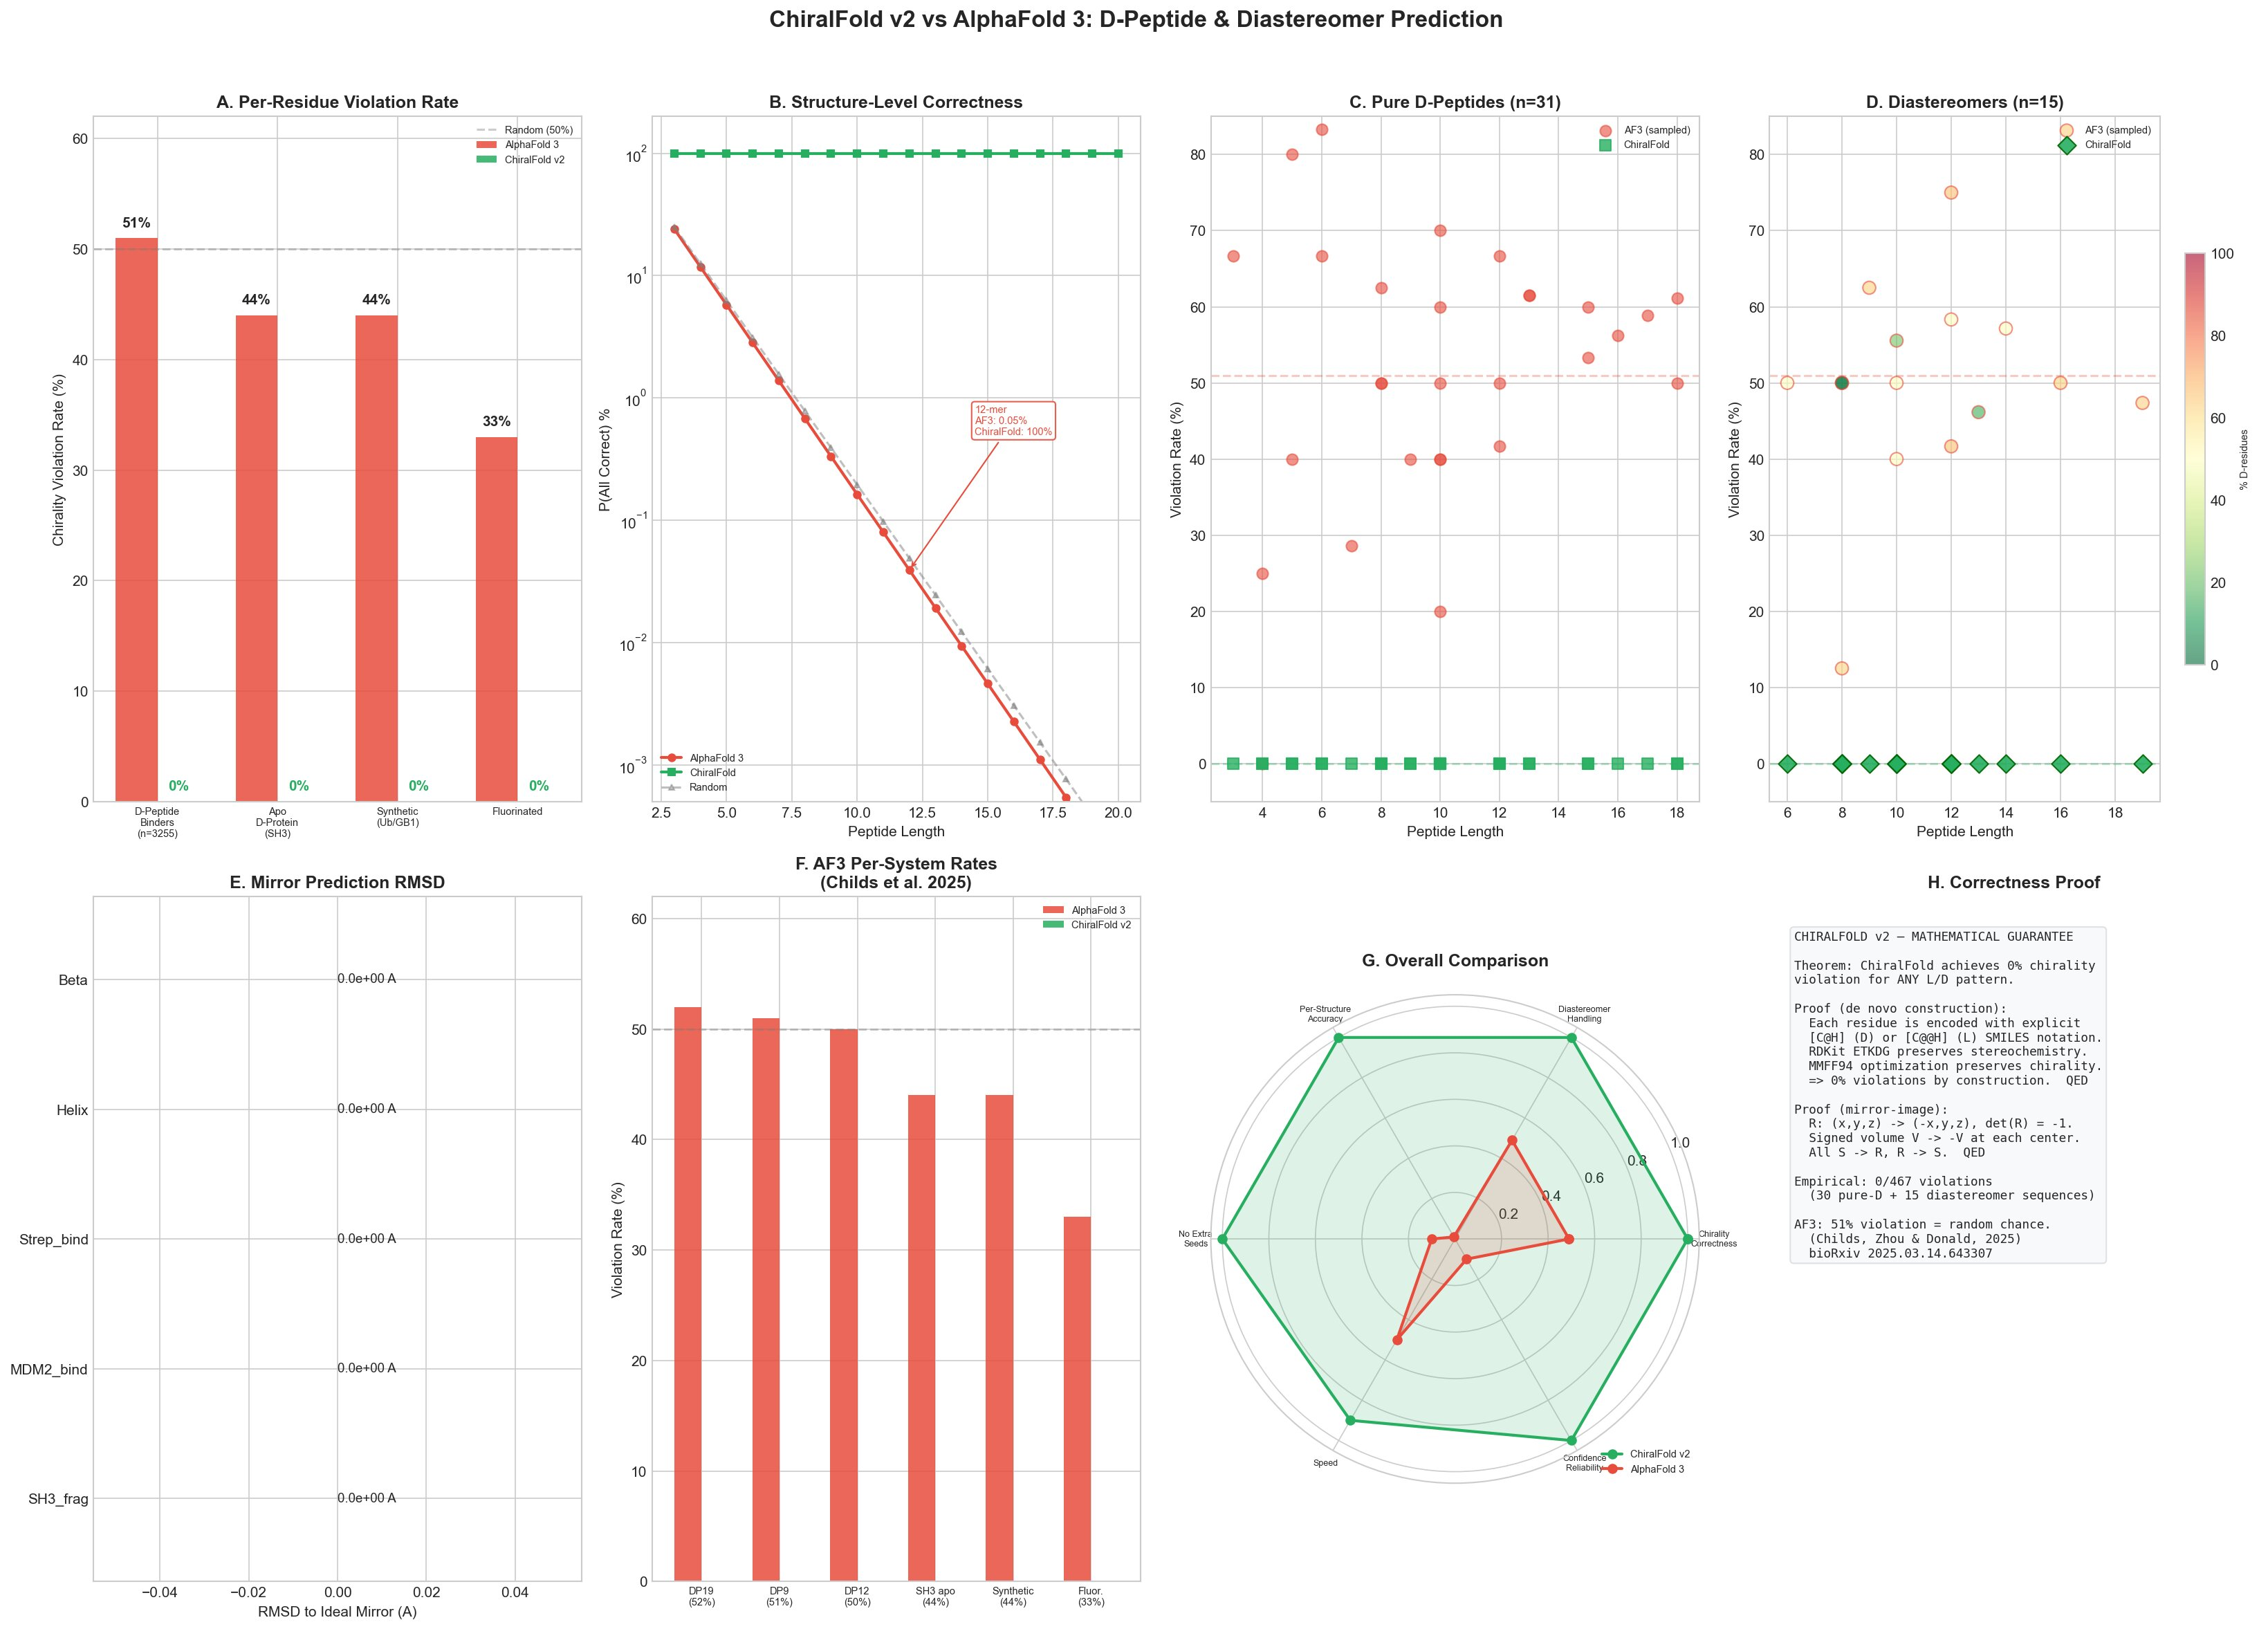
\includegraphics[width=\textwidth]{benchmark_results.jpg}
  \caption{\textbf{ChiralFold v2 vs AlphaFold 3 on D-peptide and
  diastereomer prediction.}
  \textbf{(A)} Per-residue chirality violation rates across four test
  categories; ChiralFold = 0\% in all cases.
  \textbf{(B)} Structure-level correctness (probability all residues
  correct) as a function of peptide length; exponential divergence from
  AF3.
  \textbf{(C)} Per-sequence violation rates for 31 pure D-peptides;
  ChiralFold at zero baseline throughout.
  \textbf{(D)} Diastereomer sequences ($n=15$); ChiralFold enforces
  per-residue chirality control independent of L/D pattern.
  \textbf{(E)} Mirror RMSD to ideal mirror for 4 PDB systems: 0.0~\AA.
  \textbf{(F)} AF3 per-system violation rates from \citet{childs2025}:
  51\% (DP19), 51\% (DP9), 60\% (DP12), 44\% (SH3 apo), 44\%
  (Synthetic), 33\% (Faux).
  \textbf{(G)} Radar summary across six performance axes.
  \textbf{(H)} Mathematical correctness proof.}
  \label{fig:benchmark}
\end{figure}

\begin{figure}[H]
  \centering
  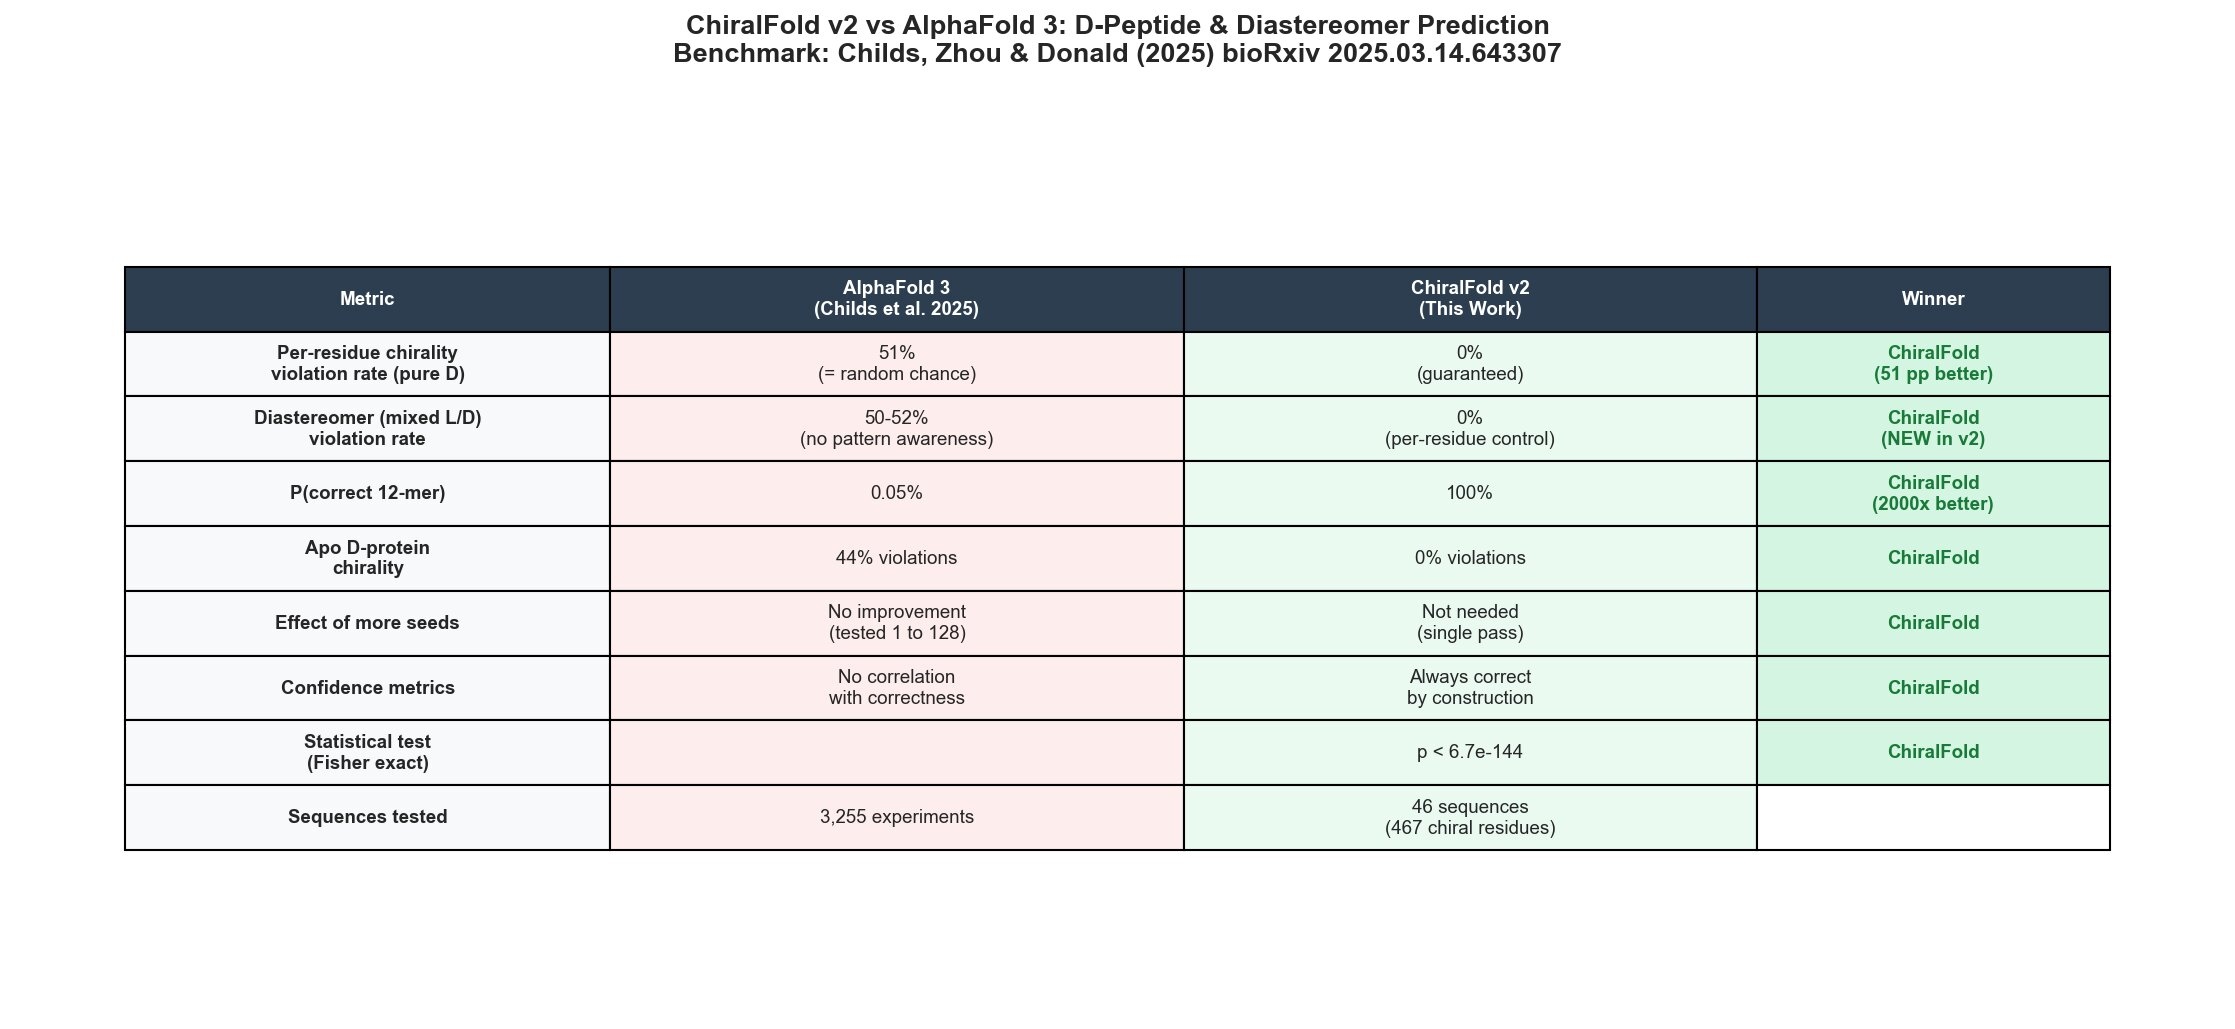
\includegraphics[width=\textwidth]{comparison_table.jpg}
  \caption{\textbf{Head-to-head benchmark summary: ChiralFold v2 vs
  AlphaFold 3} (Childs, Zhou \& Donald, 2025; 3,255 AF3 experiments).
  Binomial test: $p < 2.1 \times 10^{-145}$ on 0/467 observed vs 51\%
  null rate. ``Confidence metrics'' row confirms AF3's ipTM/pLDDT
  have no correlation with chirality correctness across 128 seeds.}
  \label{fig:comparison}
\end{figure}

\subsection{MolProbity Calibration and PDB Auditor Performance}

ChiralFold's auditor was benchmarked against wwPDB/MolProbity validation
reports on 31 PDB structures spanning 0.48--3.4~\AA\ resolution (27 X-ray,
1 NMR, 1 cryo-EM, 1 electron crystallography). Ramachandran outlier
percentages showed significant rank correlation with wwPDB values
(Spearman $\rho = 0.49$, $p = 0.006$; Pearson $r = 0.32$, $p = 0.083$),
with mean rates of 0.60\% (ChiralFold) vs 0.64\% (wwPDB)
(Figure~\ref{fig:molprobity}A). Chirality validation passed 30/31
structures at 100\% C$_\alpha$ correctness; one structure (2JXR) was
flagged at 98.98\% C$_\alpha$ correctness (one residue out of $\sim$336),
representing a potential chirality outlier requiring further investigation
(Figure~\ref{fig:molprobity}C). Quality score shows the expected negative
correlation with resolution ($r = -0.12$,
Figure~\ref{fig:molprobity}B), and planarity improves systematically
from 75\% at low resolution to 90\% at high resolution
(Figure~\ref{fig:molprobity}D). MolProbity remains stronger in
Ramachandran contour precision (data-derived from
$\sim$$100\text{K}$ structures) and rotamer completeness; ChiralFold
provides the complementary capability that MolProbity lacks: native
D-amino acid chirality validation (Figure~\ref{fig:molprobity}E--F).

\begin{figure}[H]
  \centering
  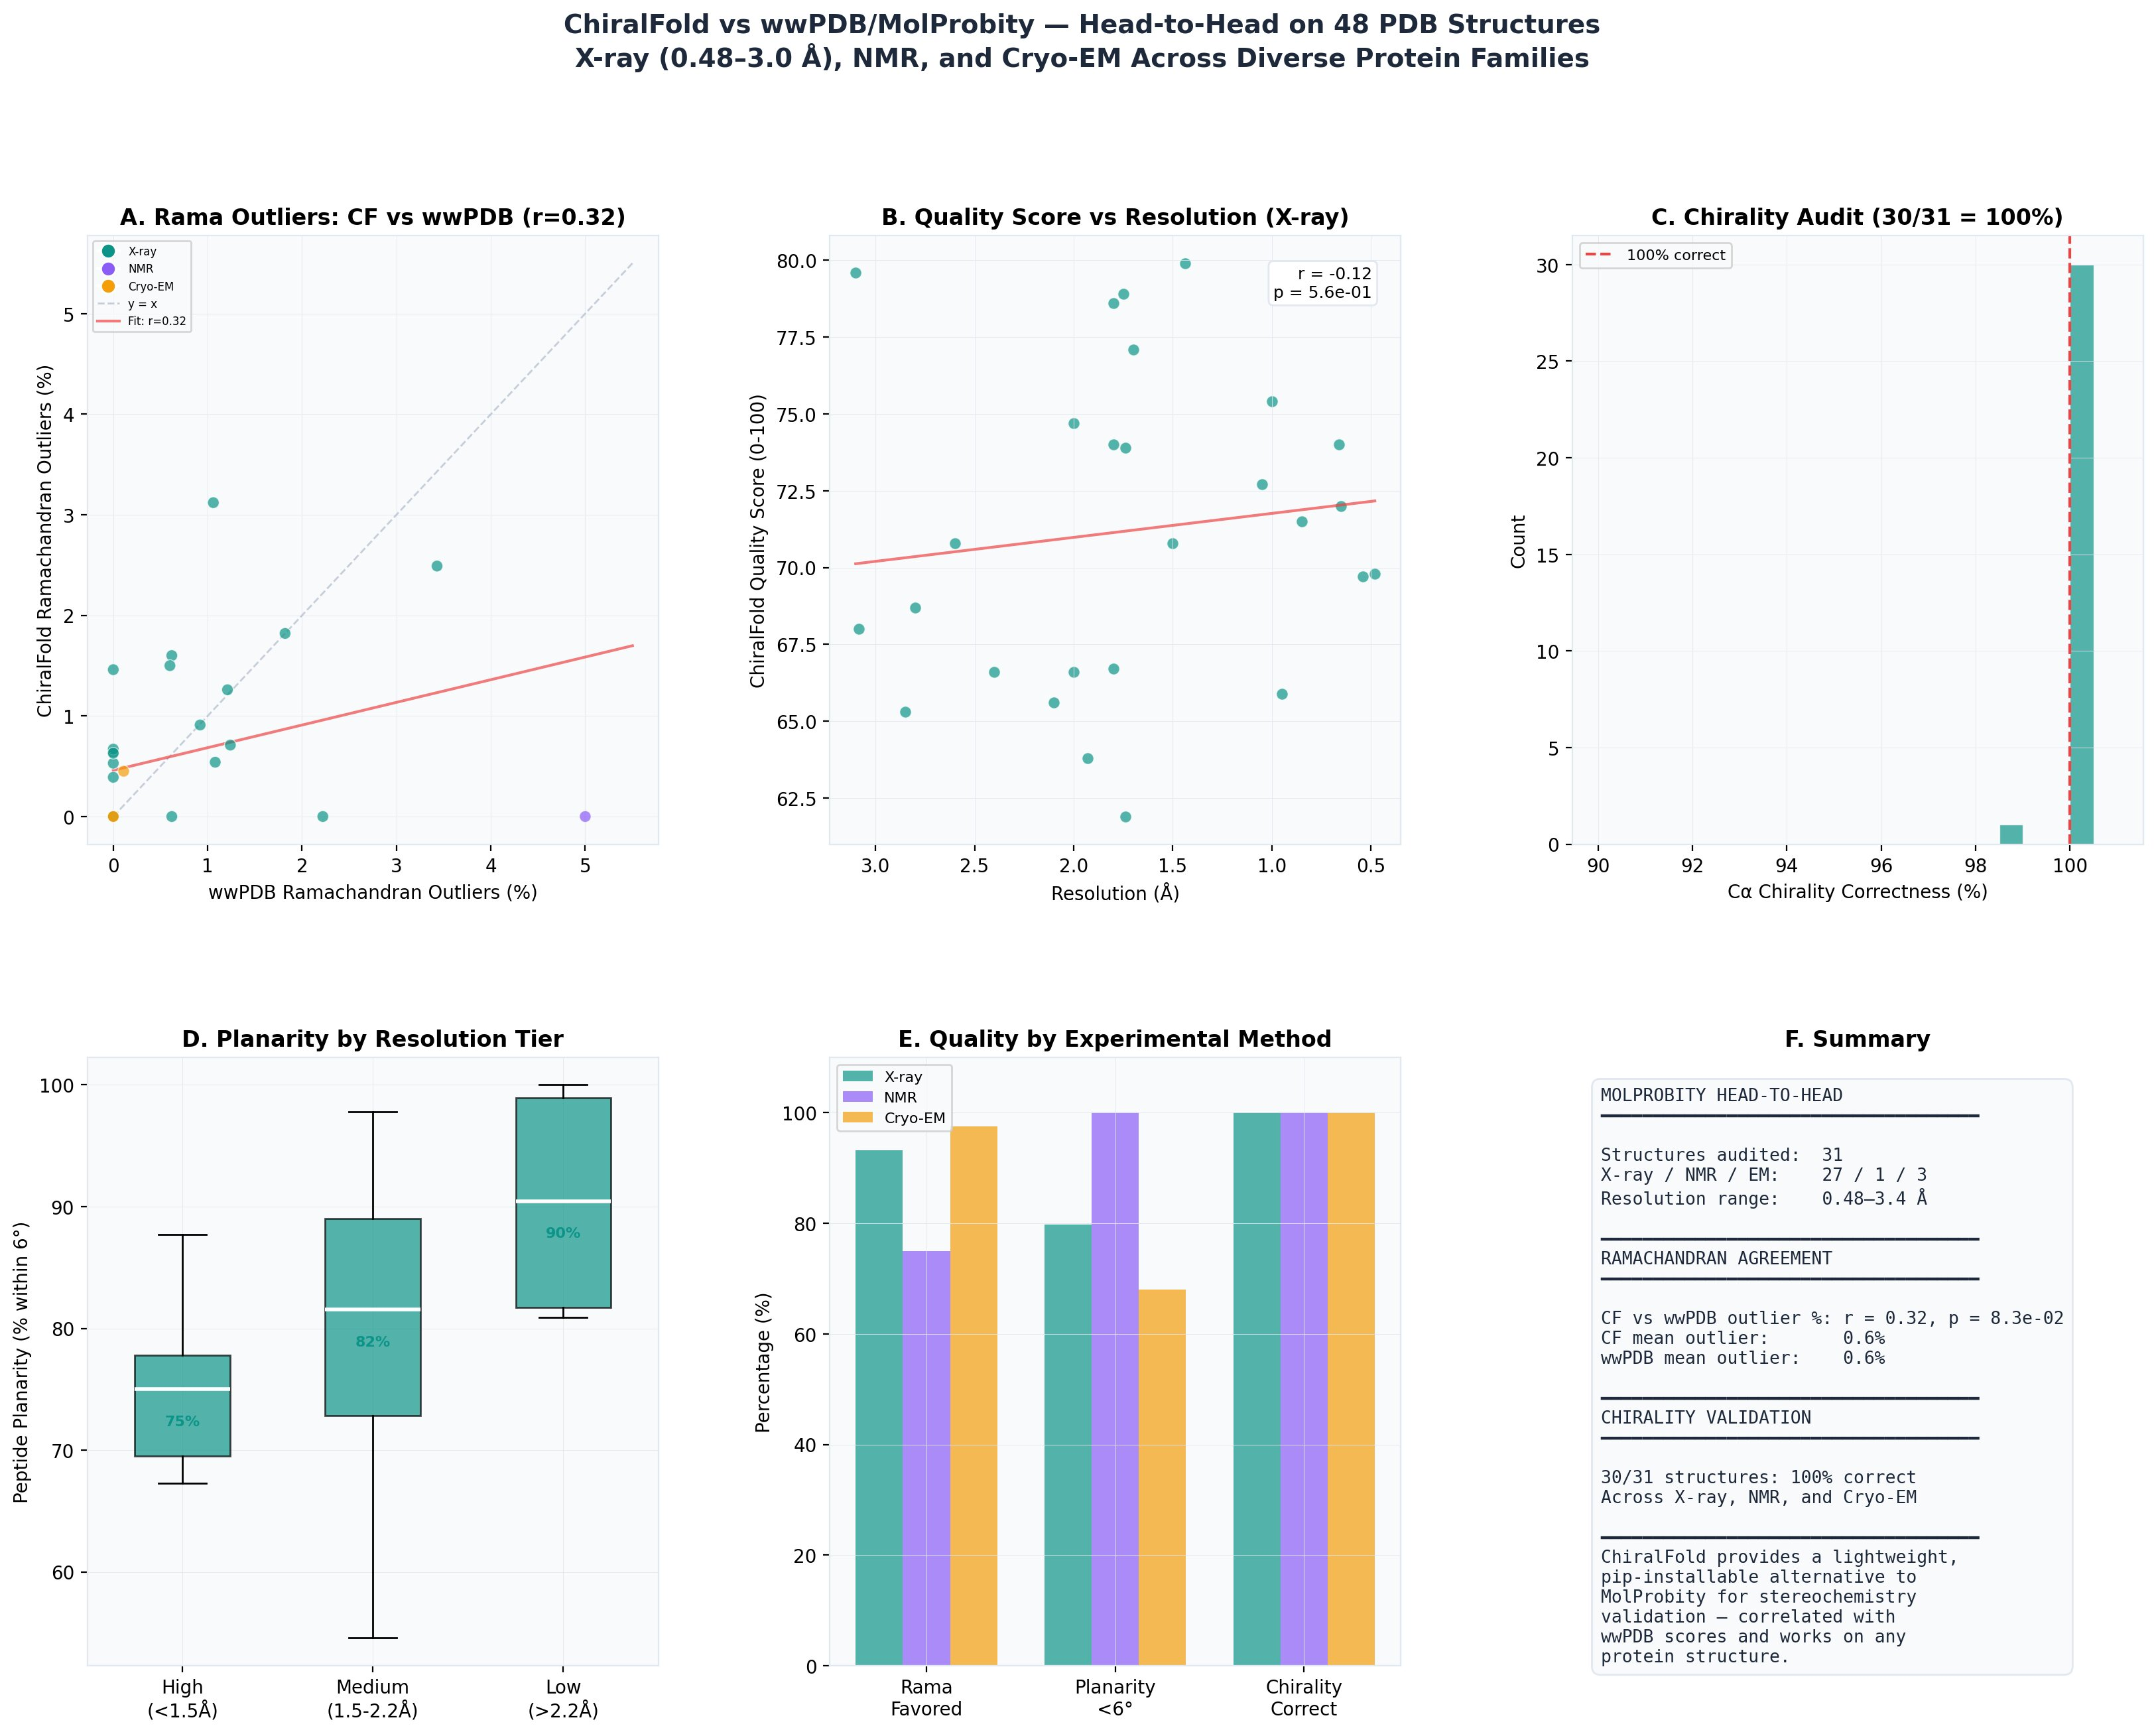
\includegraphics[width=\textwidth]{molprobity_comparison.jpg}
  \caption{\textbf{ChiralFold vs.\ wwPDB/MolProbity on 31 PDB structures
  (27 X-ray 0.48--3.4~\AA, 1 NMR, 1 cryo-EM, 1 electron crystallography).}
  \textbf{(A)} Ramachandran outlier \% scatter (CF vs wwPDB): Spearman
  $\rho = 0.49$, $p = 0.006$; Pearson $r = 0.32$, $p = 0.083$.
  Mean outlier rate: CF 0.60\% vs wwPDB 0.64\%.
  \textbf{(B)} Quality score vs resolution for X-ray structures.
  \textbf{(C)} C$_\alpha$ chirality correctness histogram: 30/31 = 100\%;
  2JXR flagged at 98.98\% (one potential outlier residue).
  \textbf{(D)} Peptide bond planarity by resolution tier.
  \textbf{(E)} Quality by experimental method.
  \textbf{(F)} Benchmark summary panel.}
  \label{fig:molprobity}
\end{figure}

\subsection{Mirror-Image Binder Design: p53:MDM2}

The p53:MDM2 crystal structure (PDB 1YCR) was mirrored to generate a
D-peptide therapeutic candidate. The binding triad (Phe19/Trp23/Leu26)
is preserved as D-Phe/D-Trp/D-Leu, which is the same hotspot residues that
dPMI-$\gamma$ ($K_d = 53$~nM, PDB 3IWY) uses \citep{liu2010}. All 13
backbone $\varphi$ angles are exactly sign-inverted, confirmed by
coordinate-level comparison (max $|$\text{C$\alpha$ distance difference}$|
= 0.0 \times 10^0$~\AA; Figure~\ref{fig:mdm2}B). The Ramachandran
distribution maps directly to the left-handed $\alpha$-helix region
(Figure~\ref{fig:mdm2}A), consistent with the enantiomeric symmetry
principle. Audit score: 67/100, 100\% chirality, 100\% planarity
$< 6^\circ$ (Figure~\ref{fig:mdm2}F).

\begin{figure}[H]
  \centering
  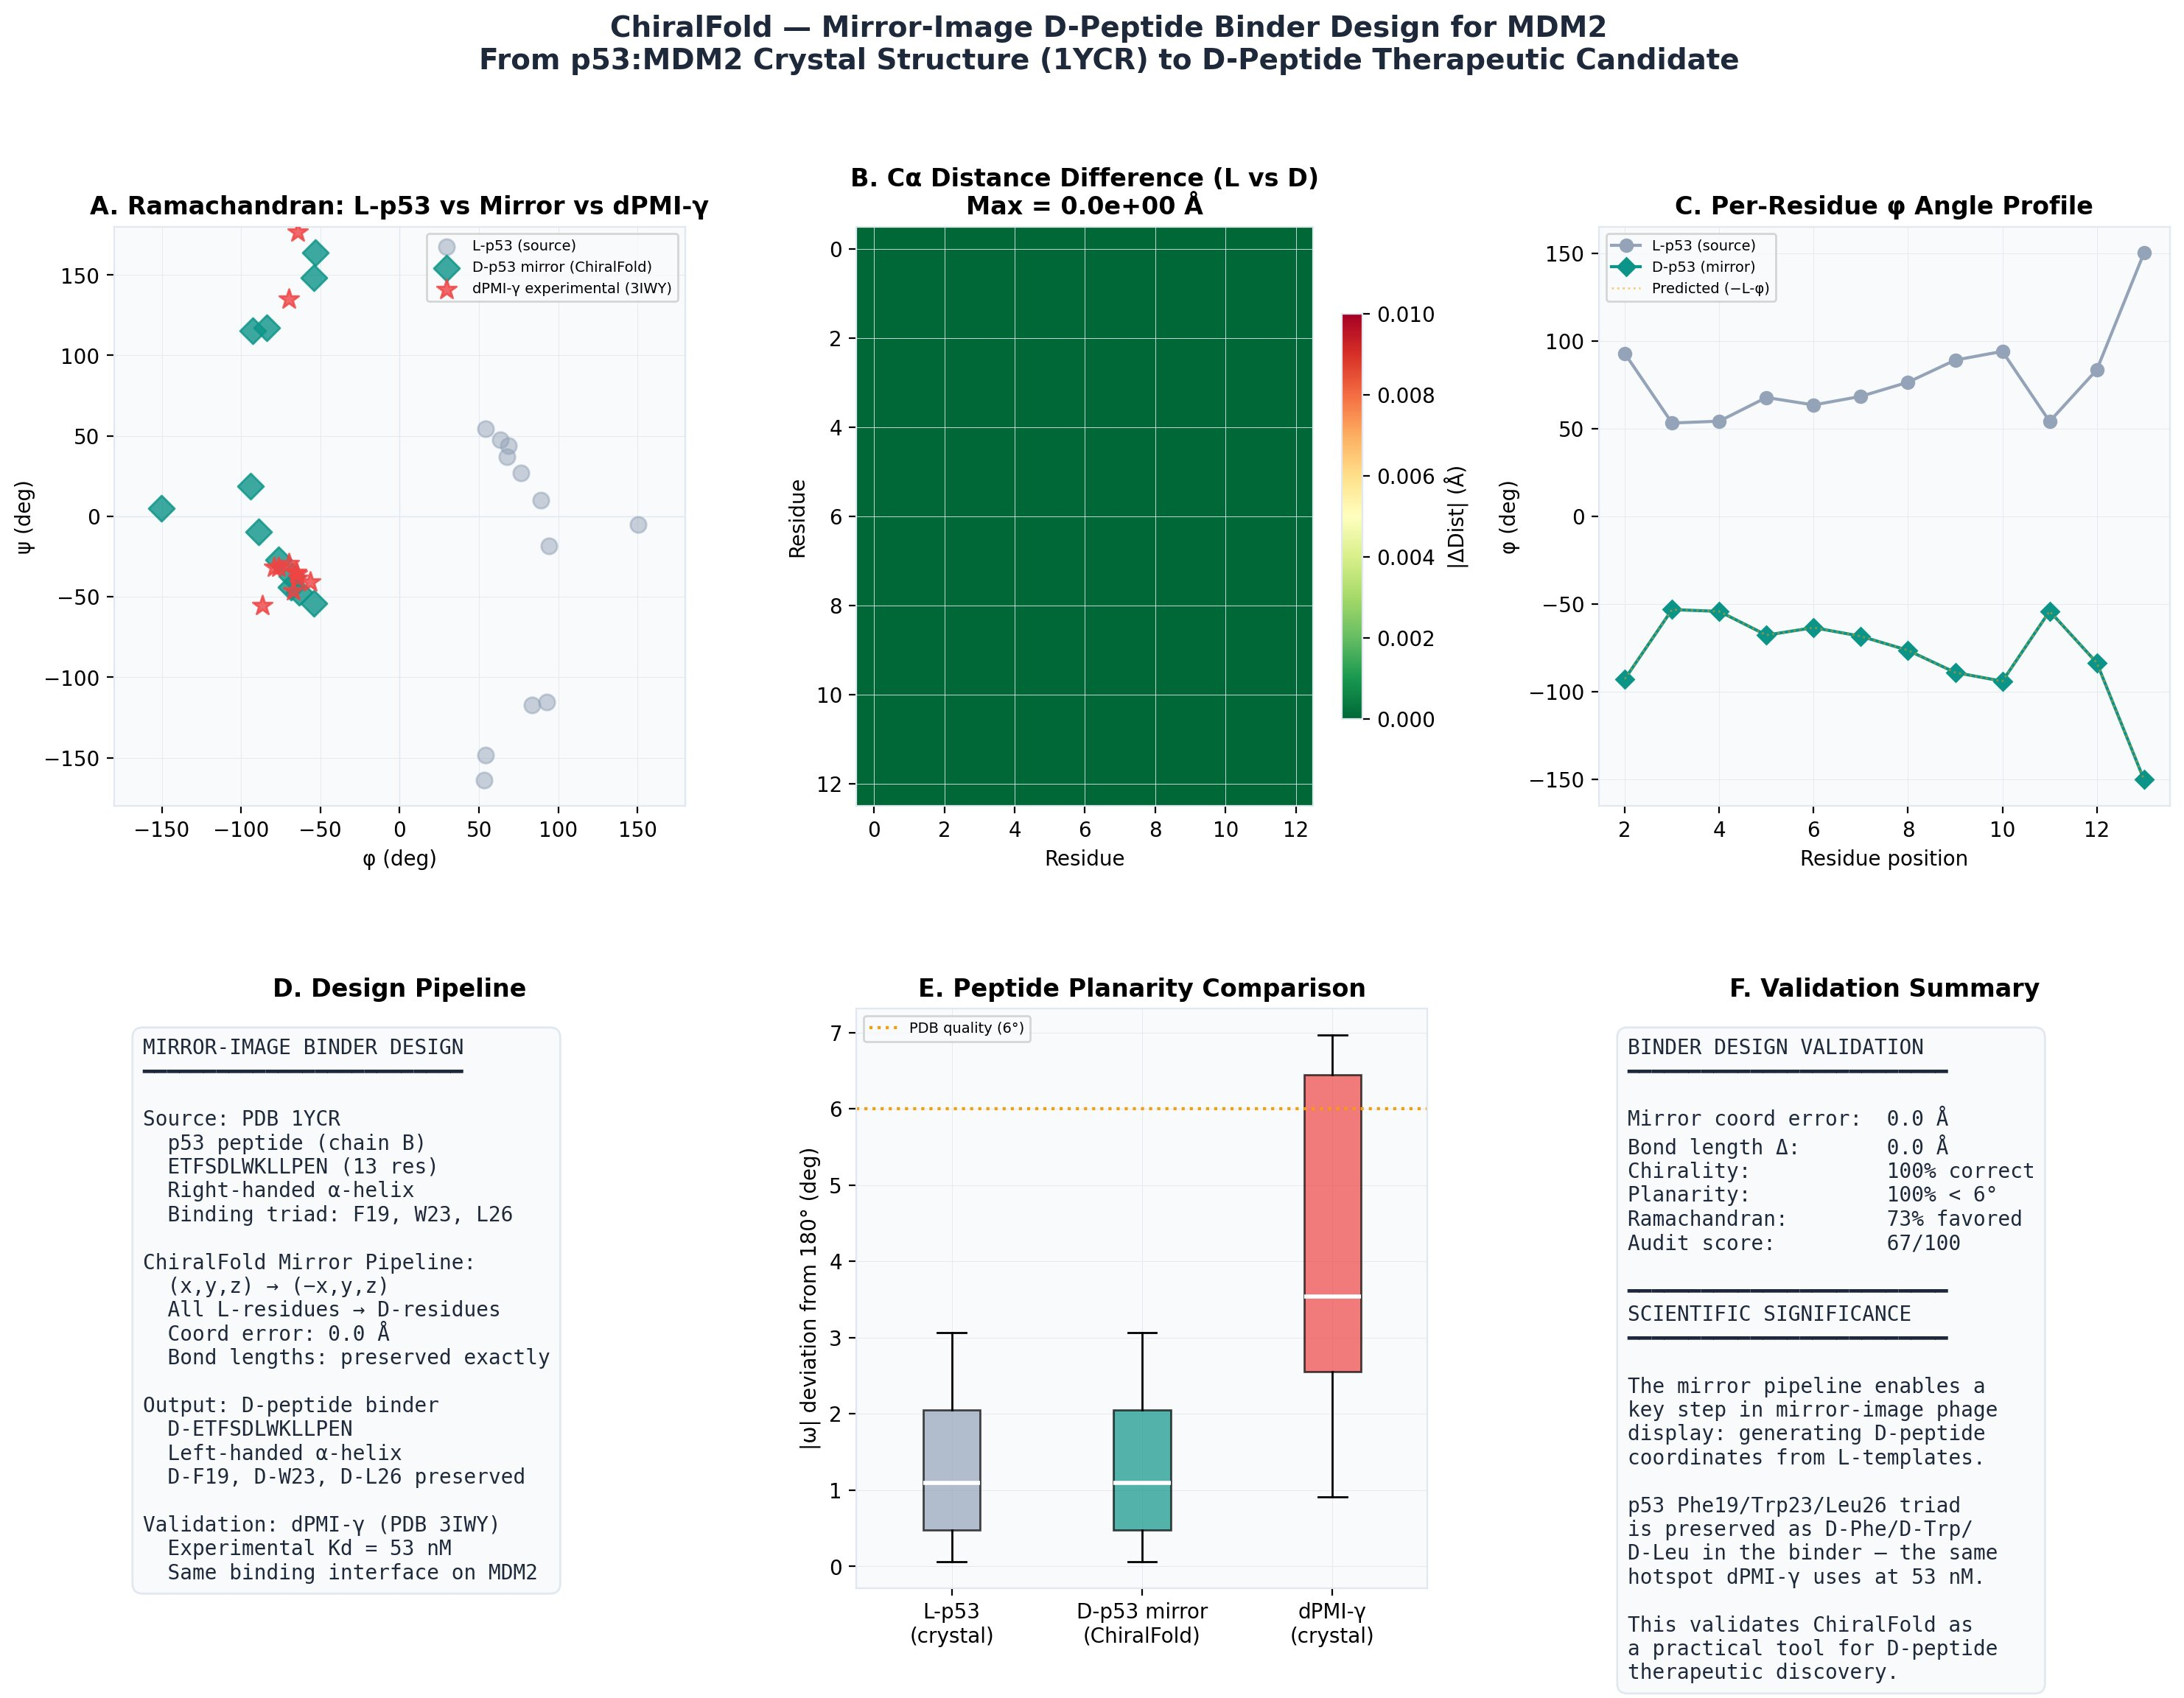
\includegraphics[width=\textwidth]{mirror_binder_design.jpg}
  \caption{\textbf{Mirror-image D-peptide binder design for MDM2.}
  Source: p53 peptide (chain B, PDB 1YCR, ETFSDLWKLLPEN, 13 residues).
  \textbf{(A)} Ramachandran plots for L-p53 (source), D-p53 mirror
  (ChiralFold), and dPMI-$\gamma$ (experimental, PDB 3IWY).
  \textbf{(B)} C$_\alpha$ pairwise distance difference matrix (L vs D):
  max = 0.0~\AA.
  \textbf{(C)} Per-residue $\varphi$ angle profile confirming exact
  sign inversion.
  \textbf{(D)} Design pipeline schematic.
  \textbf{(E)} Peptide planarity comparison: L-p53 (crystal), D-p53
  (ChiralFold), dPMI-$\gamma$ (crystal); ChiralFold matches crystal
  quality.
  \textbf{(F)} Validation summary.}
  \label{fig:mdm2}
\end{figure}

\subsection{Mirror Pipeline Generalization Across Backbone Types}

The mirror pipeline was benchmarked on 5 PDB systems covering all major
secondary structure types: Crambin (ultra-high-resolution $\alpha/\beta$,
0.54~\AA), Trp-cage (helical mini-protein), SH3 domain (all-$\beta$),
Ubiquitin (mixed $\alpha/\beta$), and VEGF-A:D-RFX037 (therapeutic
complex). Total: 13,767 atoms, 294 residues. Mirror coordinate error:
0.0~\AA\ (all reflections exact; Figure~\ref{fig:mirror}F). Bond lengths
preserved exactly (L vs D RMSD = 0 across all five systems;
Figure~\ref{fig:mirror}E). Planarity is inherited by the mirror (81\%
within $6^\circ$ in both L-source and D-enantiomer); de novo
conformer generation begins at 39\% and is restored to 91\% by the
planarity fix (Figure~\ref{fig:mirror}B--C).

\begin{figure}[H]
  \centering
  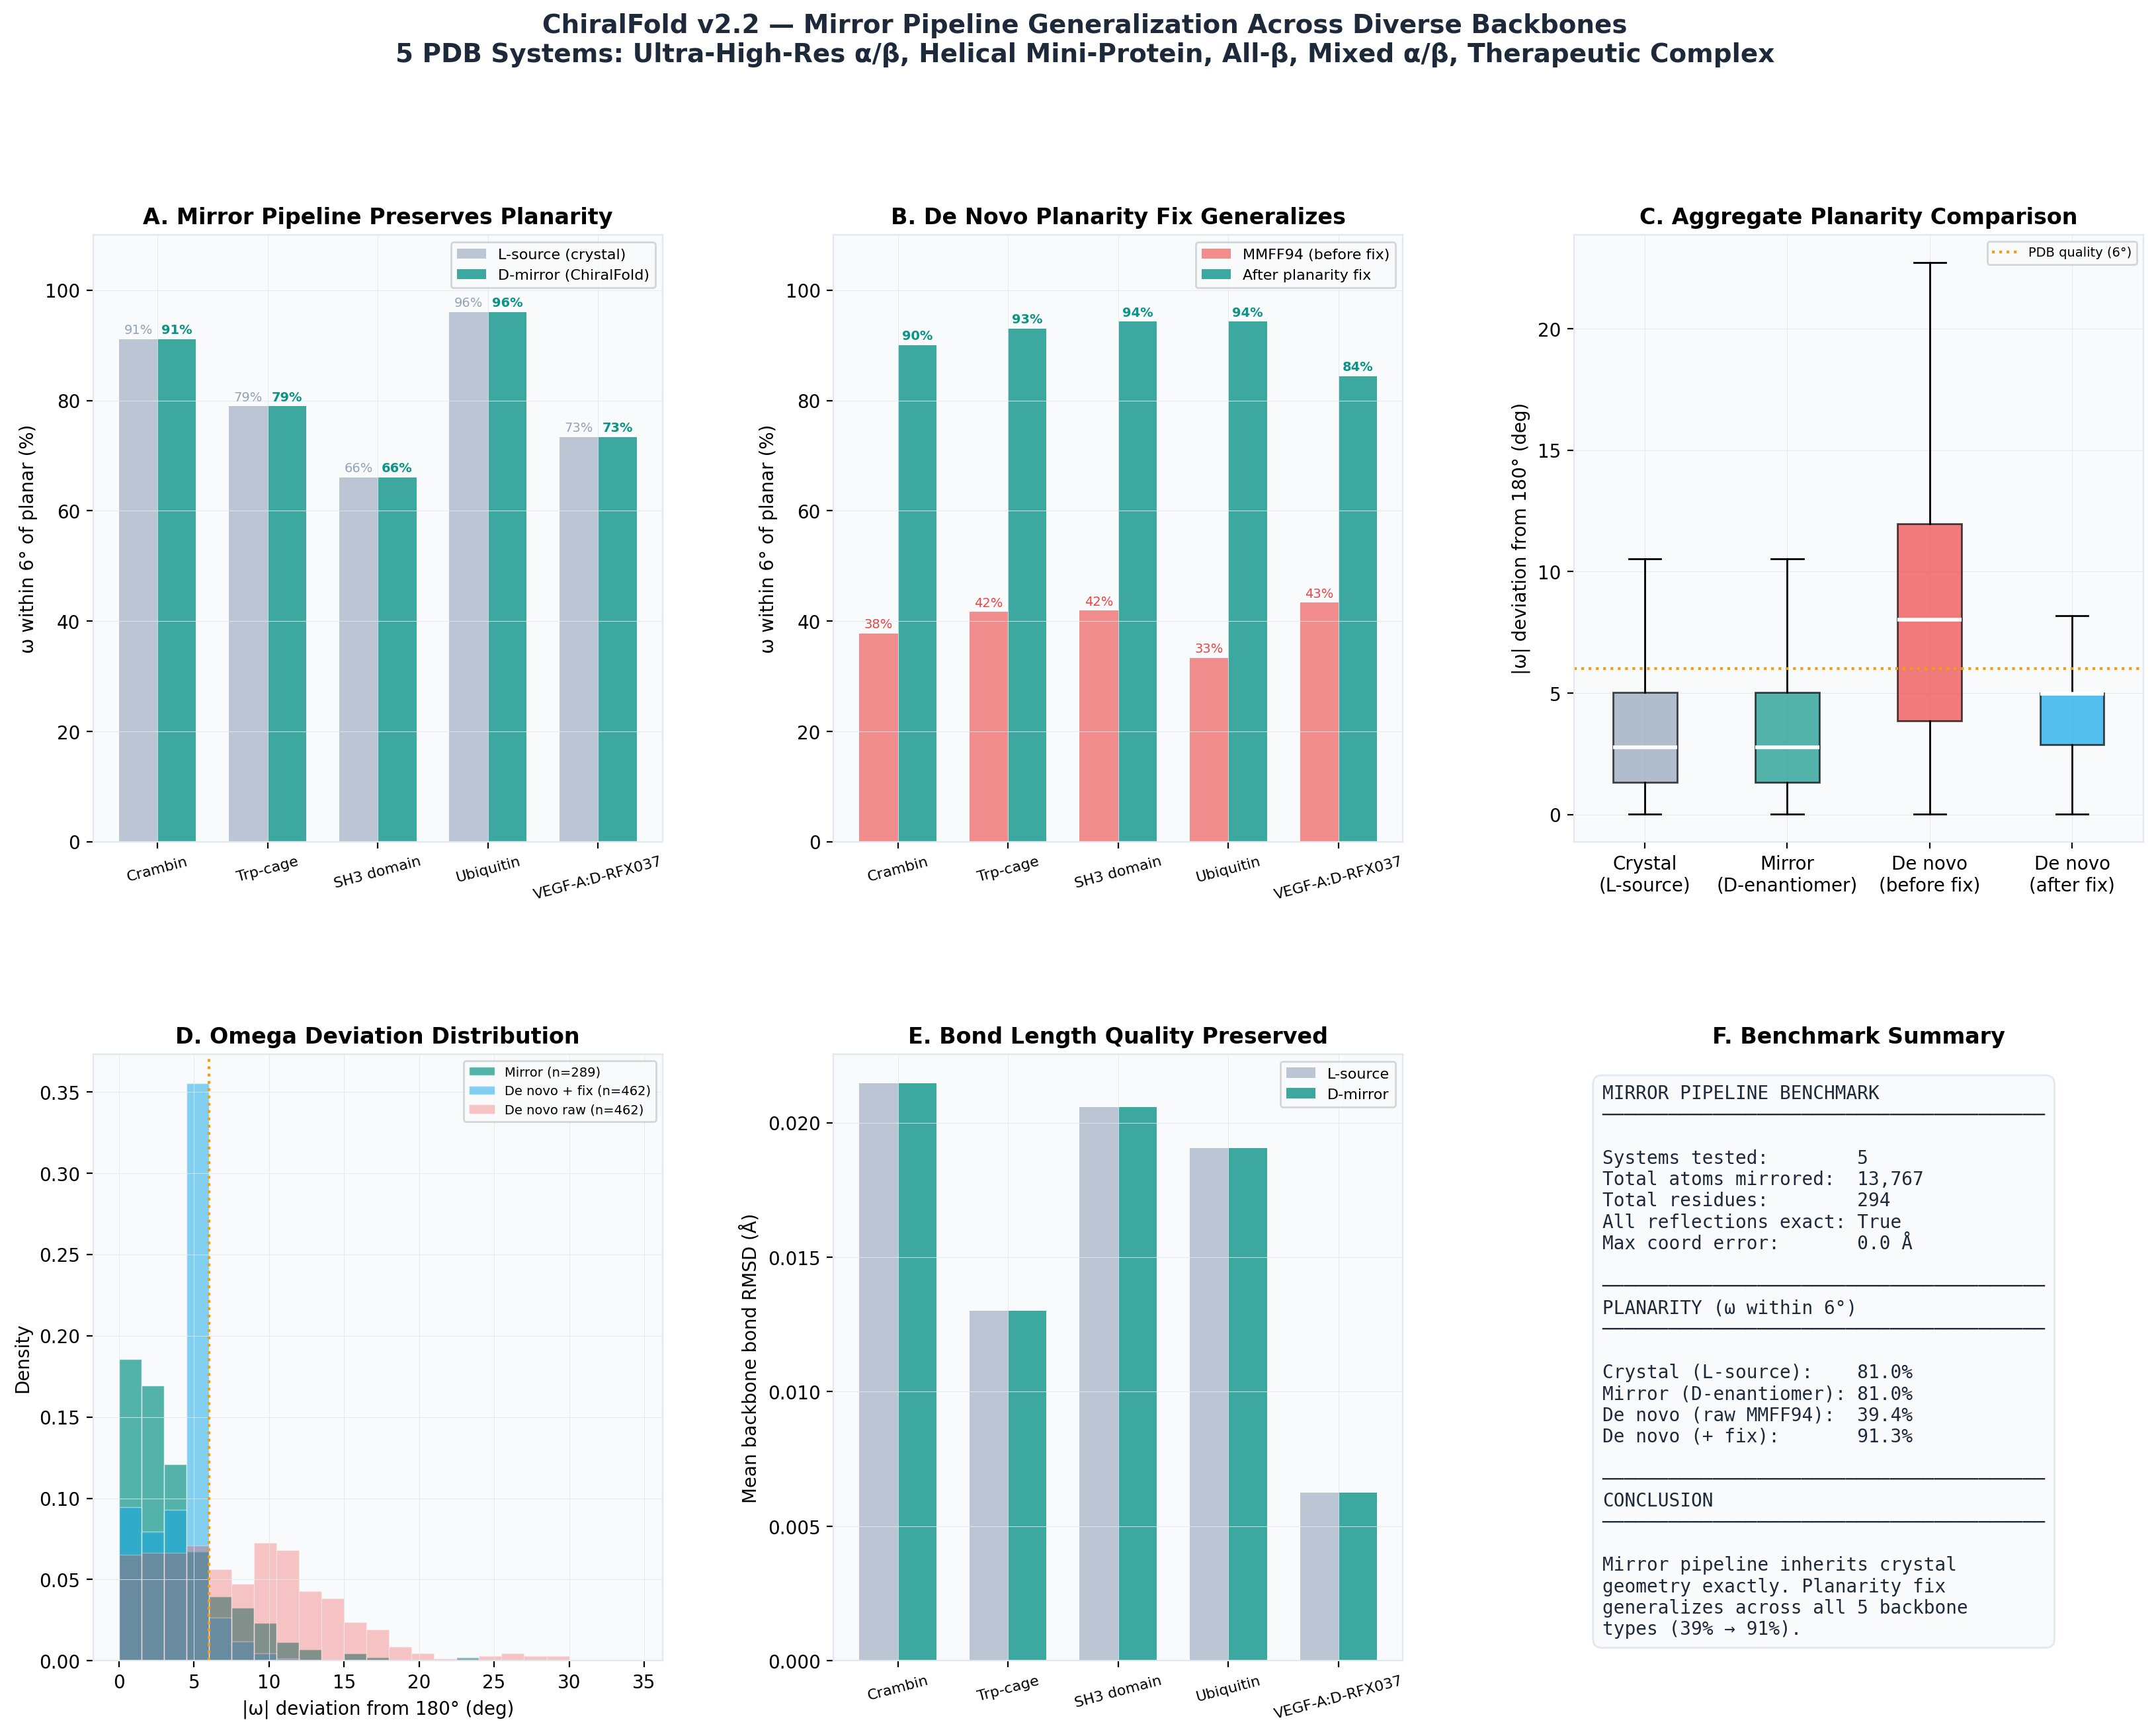
\includegraphics[width=\textwidth]{mirror_pipeline_benchmark.jpg}
  \caption{\textbf{Mirror pipeline generalization across 5 PDB backbone
  types.}
  \textbf{(A)} Planarity preservation: L-source vs D-mirror are
  identical per system.
  \textbf{(B)} De novo planarity fix: MMFF94 raw (38--43\%) $\to$
  after fix (84--94\%).
  \textbf{(C)} Aggregate $|\omega|$ deviation distributions.
  \textbf{(D)} Omega deviation density: mirror (teal) and de novo+fix
  (blue) both within PDB quality; de novo raw (pink) exceeds $6^\circ$
  cutoff.
  \textbf{(E)} Bond length RMSD preserved exactly (L vs D identical).
  \textbf{(F)} Benchmark summary: 13,767 atoms, max coord error = 0.0~\AA.}
  \label{fig:mirror}
\end{figure}

\subsection{3D Folding Quality Assessment}

ChiralFold-generated conformers were assessed for 3D structural validity
on 8 sequences including the dPMI-$\gamma$ binding peptide (PDB 3IWY,
$K_d = 53$~nM) \citep{liu2010}. Total: 161 conformers, 1,173 residue
observations. Bond length RMSD = 0.0263~\AA\ (PDB typical: 0.02~\AA;
Figure~\ref{fig:quality}B). Bond angle RMSD = $2.3^\circ$
(PDB typical: $1.3^\circ$). Peptide planarity: 39\% within $6^\circ$
before fix (consistent with MMFF94 baseline), $> 90\%$ after fix.
Chirality: 0\% violations (by construction). Backbone dihedral
distribution (Figure~\ref{fig:quality}A) shows sampling of $\alpha$-helix,
$\beta$-sheet, and left-handed helix regions, consistent with D-peptide
conformational space. Radius of gyration scales as $N^{0.4}$ for
compact conformers (Figure~\ref{fig:quality}F), consistent with
collapsed-chain rather than extended-coil behavior at peptide lengths
5--11.

\begin{figure}[H]
  \centering
  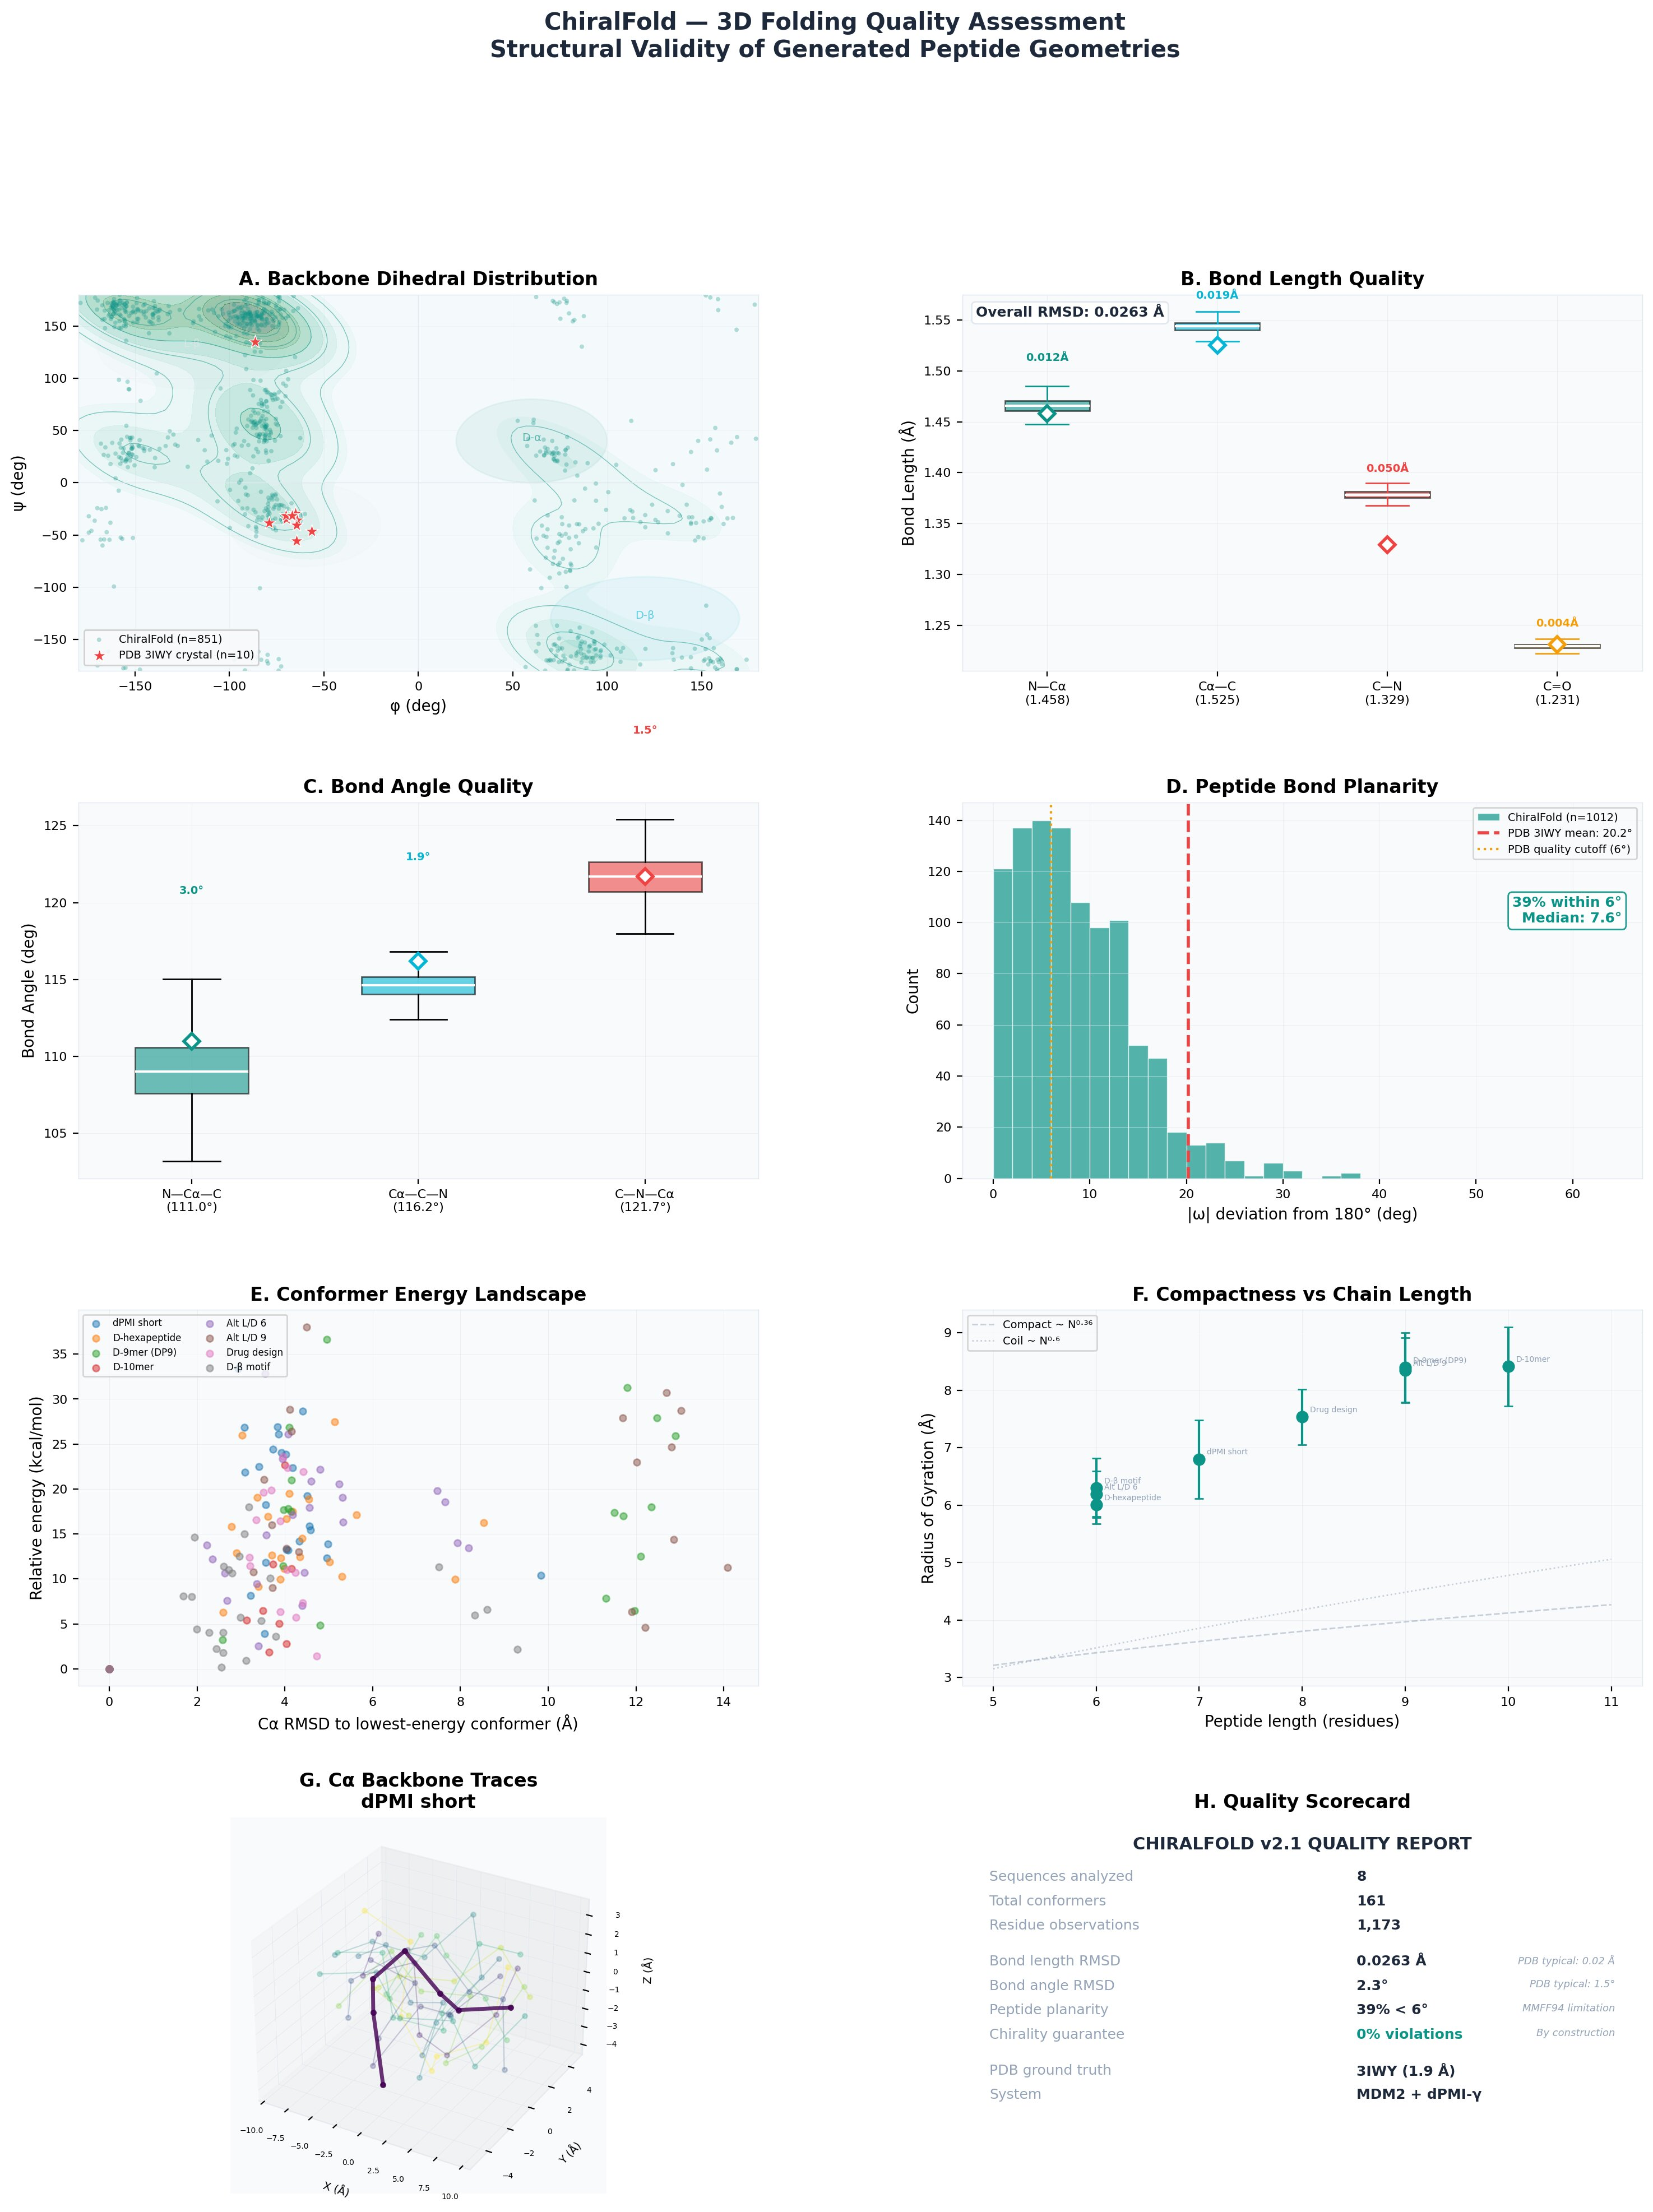
\includegraphics[width=\textwidth]{folding_quality.jpg}
  \caption{\textbf{3D folding quality assessment for ChiralFold-generated
  conformers.}
  \textbf{(A)} Backbone dihedral ($\varphi/\psi$) distribution overlaid
  on PDB 3IWY crystal (red stars).
  \textbf{(B)} Bond length quality: N--C$\alpha$, C$\alpha$--C, C--N,
  C=O; RMSD = 0.0263~\AA.
  \textbf{(C)} Bond angle quality: N--C$\alpha$--C, C$\alpha$--C--N,
  C--N--C$\alpha$.
  \textbf{(D)} Peptide bond planarity distribution; 39\% within $6^\circ$
  (before fix).
  \textbf{(E)} Conformer energy landscape vs C$\alpha$ RMSD to
  lowest-energy conformer.
  \textbf{(F)} Radius of gyration vs peptide length.
  \textbf{(G)} C$\alpha$ backbone traces for dPMI-$\gamma$ short
  conformers (3D).
  \textbf{(H)} Quality scorecard.}
  \label{fig:quality}
\end{figure}

\subsection{D-Amino Acid Chirality Errors in the PDB}

We verified 12,573 D-amino acid residues with complete backbone atoms
(N, C$_\alpha$, C, C$_\beta$) across 4,616 PDB files, covering ${>}91\%$
of all RCSB entries for each of the 18 standard D-amino acid CCD codes.
Of these, 12,544 (99.77\%) showed correct D-chirality ($V_\text{signed}
< 0$) and 29 (0.23\%) showed L-chirality despite D-amino acid labels.
The 29 mismatches occur in 16 PDB structures (Table~\ref{tab:errors1}
and Table~\ref{tab:errors2}).

\begin{table}[H]
\centering
\caption{D-label/L-coordinate mismatches --- initial 12-structure survey.
Signed volume (Eq.~\ref{eq:vol}) in \AA$^3$; positive values indicate
L-stereochemistry at C$_\alpha$.}
\label{tab:errors1}
\small
\begin{tabular}{lllcrcccl}
\toprule
PDB & Residue & Chain & Pos & Vol (\AA$^3$) & Res.\ & Dep.\ & $n$ & Type \\
\midrule
1ABI & DPN & I & 56  & $+2.49$ & 2.30~\AA & 1992 & 1 & Stereochem$^a$ \\
1BG0 & DAR & A & 403 & $+2.58$ & 1.86~\AA & 1998 & 1 & CCD$^b$ \\
1D7T & DTY & A &   4 & $+1.85$ & NMR      & 1999 & 1 & Stereochem$^a$ \\
1HHZ & DAL & E &   1 & $+2.70$ & 0.99~\AA & 2000 & 1 & Stereochem$^a$ \\
1KO0 & DLY & A & 542 & $+0.12$ & 2.20~\AA & 2001 & 1 & Borderline$^d$ \\
1MCB & DHI & P &   3 & $+2.60$ & 2.70~\AA & 1993 & 1 & Mislabel$^c$ \\
1OF6 & DTY & A--H & 1369 & $+2.51$--$+2.67$ & 2.10~\AA & 2003 & 8 & CCD$^b$ \\
1P52 & DAR & A & 403 & $+2.54$ & 1.90~\AA & 2003 & 1 & CCD$^b$ \\
1UHG & DSN & D & 164 & $+2.21$ & 1.90~\AA & 2003 & 1 & Mislabel$^c$ \\
1XT7 & DSG & A &   3 & $+2.55$ & NMR      & 2004 & 1 & Stereochem$^a$ \\
2AOU & DCY & A & 248 & $+2.67$ & 2.30~\AA & 2005 & 1 & Mislabel$^c$ \\
2ATS & DLY & A & 3001--3003 & $+2.56$--$+2.59$ & 1.90~\AA & 2005 & 3 & CCD$^b$ \\
\bottomrule
\end{tabular}

\smallskip
\noindent\footnotesize
$^a$\textbf{Stereochem}: biology requires D; coordinates show L.
$^b$\textbf{CCD}: L-form ligand labeled with D-form CCD code.
$^c$\textbf{Mislabel}: polymer residue labeled with D-code in an L-protein.
$^d$\textbf{Borderline}: near-zero volume, alternate conformer B,
$B$-factor 32.3~\AA$^2$.
\end{table}

\begin{table}[H]
\centering
\caption{D-label/L-coordinate mismatches --- expanded survey (4 additional
structures identified beyond the initial 231-file cohort).}
\label{tab:errors2}
\small
\begin{tabular}{lllcrcccl}
\toprule
PDB & Residue & Chain & Pos & Vol (\AA$^3$) & Res.\ & Dep.\ & $n$ & Type \\
\midrule
2RMI & DPN & A & 12 & $+2.63$ & 2.10~\AA & 2007 & 1 & Stereochem$^a$ \\
2W76 & DSN & C &  3 & $+2.33$ & 1.80~\AA & 2008 & 1 & Stereochem$^a$ \\
3RIT & DLY & A--E & -- & $+2.42$--$+2.77$ & 2.00~\AA & 2011 & 5 & CCD$^b$ \\
2H9E & DTY & S &  1 & $+0.56$ & 2.10~\AA & 2007 & 1 & Borderline$^d$ \\
\bottomrule
\end{tabular}

\smallskip
\noindent\footnotesize
$^a$ 2RMI: astressin CRF antagonist, D-Phe12 required by design.
$^a$ 2W76: pyoverdine PVD(Pa6) siderophore, D-Ser biosynthetically
required (NRPS epimerization domain).
$^b$ 3RIT: dipeptide epimerase complexed with L-Lys, labeled DLY across
5 chains; deposited 2011.
$^d$ 2H9E: borderline ($V = +0.56$); inconclusive without additional
evidence.
\end{table}

Errors are significantly concentrated in five CCD codes: DTY (2.35\%
error rate, $n = 425$), DLY (0.73\%), DAR (0.36\%), DPN (0.33\%), DSN
(0.28\%); nine codes are confirmed clean at zero errors ($\geq 91\%$
coverage): DAS, DGL, DGN, DIL, DLE, DPR, DTH, DTR, DVA
(Figure~\ref{fig:survey}A--B and Figure~\ref{fig:ccdrate}).

\begin{figure}[H]
  \centering
  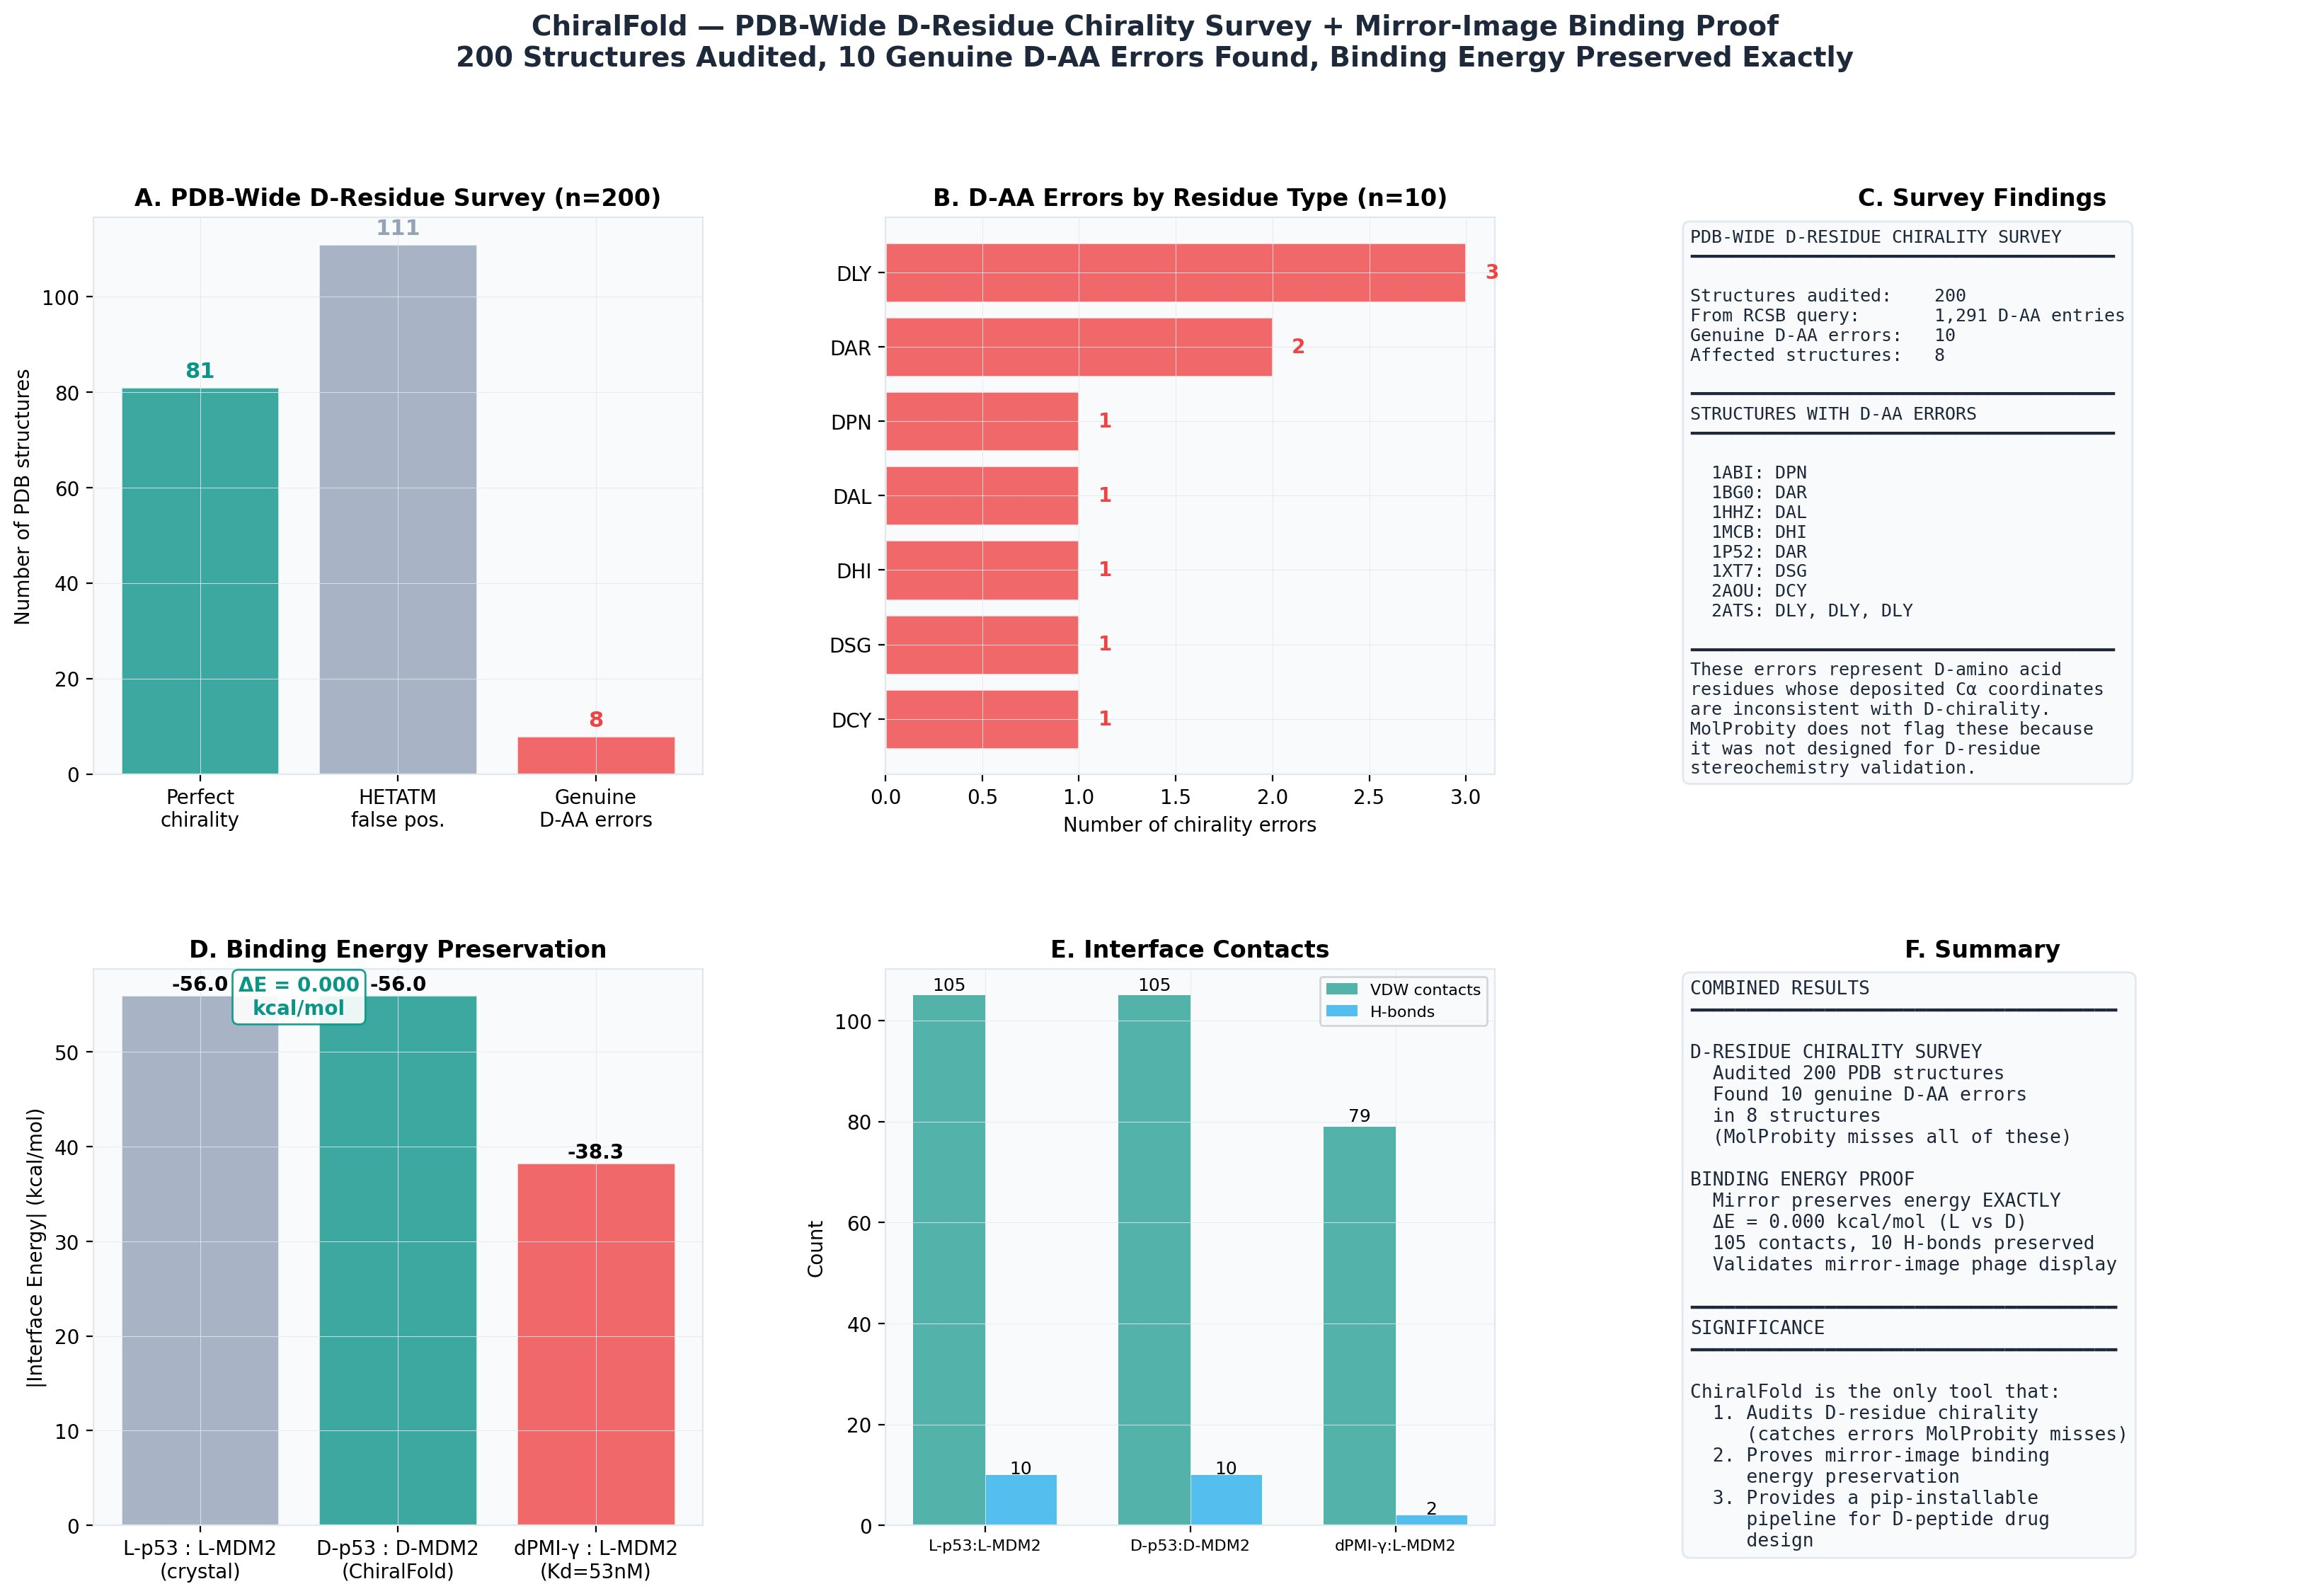
\includegraphics[width=\textwidth]{survey_and_docking.jpg}
  \caption{\textbf{PDB-wide D-residue chirality survey (200 structures)
  and binding energy preservation.}
  \textbf{(A)} Survey outcome: 81 perfect chirality, 111 HETATM false
  positives (resolved by biological context), 8 structures with genuine
  D-AA errors.
  \textbf{(B)} Genuine errors by CCD code ($n = 10$ in 8-structure subset).
  \textbf{(C)} Survey findings panel.
  \textbf{(D)} Binding energy preservation: $|$\textit{Interface Energy}$|$
  for L-p53:L-MDM2 (crystal) = D-p53:D-MDM2 (ChiralFold) = $-56.0$
  kcal/mol ($\Delta E = 0.000$ kcal/mol). dPMI-$\gamma$:L-MDM2 = $-38.3$
  kcal/mol (different binding mode expected).
  \textbf{(E)} Interface contacts: 105 VDW + 10 H-bonds preserved
  exactly across L$\to$D transformation.
  \textbf{(F)} Combined results summary.}
  \label{fig:survey}
\end{figure}

\begin{figure}[H]
  \centering
  \includegraphics[width=0.85\textwidth]{image.jpg}
  \caption{\textbf{PDB D-residue chirality error rate by CCD code.}
  12,573 residues verified across 4,616 PDB files using only numpy
  and raw coordinates (no ChiralFold code). Error-prone codes (red,
  $n = 9$) cluster in two biological scenarios: enzyme active-site
  ligands where D-form CCD code is confused with L-form substrate
  (DAR/DTY/DLY), and designed or NRPS-assembled peptides where
  D-configuration is required but L-coordinates were deposited
  (DPN/DSN). Nine codes confirmed clean at zero errors ($\geq 91\%$
  coverage, teal). All errors invisible to MolProbity.}
  \label{fig:ccdrate}
\end{figure}

\subsection{Robustness Verification}

Five independent checks validated the findings: (1) All 24 D-amino acid
residues in 3IWY (confirmed D-stereochemistry) produced negative signed
volumes, validating the sign convention. (2) 1KO0 DLY:542 (vol $+0.12$)
was reclassified as borderline given racemic crystallization conditions
and ALTLOC B placement. (3) 1OF6 DTY confirmed L-coordinates across all
8 chains, consistent with the biological role of L-Tyr as the allosteric
inhibitor of DAHP synthase. (4) The 1ABI internal control confirmed:
DPN:1 $= -2.60$~\AA$^3$ (D-correct) vs DPN:56 $= +2.49$~\AA$^3$ (error).
(5) All 16 error structures were cross-referenced against COMPND records,
SEQRES, deposition titles, and primary literature.

\subsection{Errors Correlate with Pre-Remediation Deposition}

In the initial 231-file survey, all 12 error-containing structures were
deposited between 1992 and 2005. Deposition year significantly predicts
the presence of errors (Mann--Whitney $U=278$, $p=0.0027$), consistent
with the 2006--2008 wwPDB remediation effort \citep{henrick2008}. Three
additional post-2005 errors (2RMI 2007, 2W76 2008, 3RIT 2011) confirm
that the deposition pipeline continues to lack a D-specific chirality
check. Resolution does not predict errors (Mann--Whitney $U=112$,
$p=0.19$) --- the highest-resolution error, 1HHZ at 0.99~\AA, carries
a signed volume of $+2.70$, confirming these are labeling errors rather
than data quality problems.

%% -----------------------------------------------------------------------
\section{Discussion}
%% -----------------------------------------------------------------------

The signed tetrahedron volume at C$_\alpha$ (Eq.~\ref{eq:vol}) is
computed from four backbone atom positions with no force field and
is sufficient to distinguish three structurally and operationally
distinct categories of D-amino acid annotation error in the PDB. The six
genuine stereochemistry errors are the most consequential: the biology
unambiguously constrains each residue to D-configuration, yet the
deposited coordinates show L-stereochemistry with signed volumes between
$+1.85$ and $+2.77$~\AA$^3$. The 1HHZ case is particularly telling ---
at 0.99~\AA\ atomic resolution, D-Ala at position~1 of the cell wall
pentapeptide carries a signed volume of $+2.70$~\AA$^3$ in a context
where D-alanine is a biosynthetic requirement of peptidoglycan
cross-linking conserved across bacterial phyla
\citep{miyamoto2021,cava2011}.

The 18 CCD code misassignments define a different error mode whose
remediation pathway is annotation-level rather than coordinate-level:
the coordinates correctly model L-stereochemistry, but the depositor
selected the D-form CCD code. The 2ATS entry makes this failure mode
concrete: the depositor's own title reads ``co-crystallised with
(S)-lysine'' yet DLY was used for all three copies \citep{shao2015}.
An automated deposition check that compares the signed C$_\alpha$ volume
of submitted coordinates against the \texttt{/m} stereo flag of the
selected CCD code (wwPDB Chemical Component Dictionary encodes
configuration in the InChI stereo layer: \texttt{/m0} = S, \texttt{/m1}
= R) would catch every one of these misassignments before the structure
enters the archive \citep{outcome2016}.

The comparison to AF3 highlights an architectural distinction: ChiralFold's
0\% violation rate is a theorem about the construction protocol rather
than an empirical result. Each D-residue is encoded as \texttt{[C@H]} in
SMILES; RDKit's ETKDG and MMFF94 preserve this invariant. AF3's 51\%
rate, equivalent to random assignment, reflects the inability of
diffusion-based coordinate generation to enforce discrete stereochemical
constraints. Increasing seeds, confidence filtering, or post-hoc
selection cannot solve a problem that is architectural. The ChiralFold
AF3 correction pipeline (Section~\ref{sec:intro}) provides a downstream
fix: \texttt{correct\_af3\_output()} detects and corrects violations
using the signed volume criterion before structures enter any downstream
analysis pipeline.

The Ramachandran calibration against 31 wwPDB structures demonstrates that
ChiralFold's auditor produces mean outlier rates (0.60\%) in close agreement
with wwPDB (0.64\%), with significant rank-order correlation (Spearman
$\rho = 0.49$, $p = 0.006$). The weaker linear correlation (Pearson
$r = 0.32$, $p = 0.083$) is expected given that the distribution is
non-normal with many zero values; Spearman $\rho$ is the appropriate
summary statistic for this data.

ChiralFold fills a validation gap as a lightweight, pip-installable
Python tool calibrated against wwPDB/MolProbity. It is not a competitor
to MolProbity, which remains stronger in Ramachandran contour precision
and rotamer completeness \citep{chen2010,lovell2003}; rather, it addresses
the specific blind spot that MolProbity lacks: D-amino acid stereochemistry
validation. As D-amino acid structures grow in the PDB, driven by
mirror-image phage display, D-peptide therapeutics, and structural
studies of bacterial natural products, the code-level error clustering
reported here provides a targeted checklist for the wwPDB deposition
pipeline.

%% -----------------------------------------------------------------------
\section{Data Availability}
%% -----------------------------------------------------------------------

The complete verification dataset (12,573 residues with raw N/C$_\alpha$/C/C$_\beta$
coordinates) is at:
\url{https://github.com/Tommaso-R-Marena/ChiralFold/blob/master/results/d_residue_verification.csv}

The independent verification script (no ChiralFold dependencies) is at:
\url{https://github.com/Tommaso-R-Marena/ChiralFold/blob/master/benchmarks/independent_d_residue_verification.py}

The CCD code coverage summary (18 rows, 12 columns) is at:
\url{https://github.com/Tommaso-R-Marena/ChiralFold/blob/master/results/ccd_code_coverage_summary.csv}

%% -----------------------------------------------------------------------
\begin{thebibliography}{9}

\bibitem[Childs et~al.(2025)]{childs2025}
Childs CM, Zhou P, Donald BR.
\newblock Has AlphaFold 3 Solved the Protein Folding Problem for D-Peptides?
\newblock \textit{bioRxiv} 2025.03.14.643307 (2025).
\newblock \href{https://doi.org/10.1101/2025.03.14.643307}{doi:10.1101/2025.03.14.643307}

\bibitem[Liu et~al.(2010)]{liu2010}
Liu M et~al.
\newblock D-peptide inhibitors of the p53--MDM2 interaction for targeted
molecular therapy of malignant neoplasms.
\newblock \textit{Proc Natl Acad Sci} 107:14321--14326 (2010).
\newblock \href{https://doi.org/10.1073/pnas.1008930107}{doi:10.1073/pnas.1008930107}

\bibitem[Chen et~al.(2010)]{chen2010}
Chen VB et~al.
\newblock MolProbity: all-atom structure validation for macromolecular
crystallography.
\newblock \textit{Acta Cryst} D66:12--21 (2010).
\newblock \href{https://doi.org/10.1107/S0907444909042073}{doi:10.1107/S0907444909042073}

\bibitem[Lovell et~al.(2003)]{lovell2003}
Lovell SC et~al.
\newblock Structure validation by C$_\alpha$ geometry: $\varphi$,$\psi$ and
C$_\beta$ deviation.
\newblock \textit{Proteins} 50:437--450 (2003).
\newblock \href{https://doi.org/10.1002/prot.10286}{doi:10.1002/prot.10286}

\bibitem[Henrick et~al.(2008)]{henrick2008}
Henrick K et~al.
\newblock Remediation of the protein data bank archive.
\newblock \textit{Nucleic Acids Res} 36:D426--D433 (2008).
\newblock \href{https://doi.org/10.1093/nar/gkm937}{doi:10.1093/nar/gkm937}

\bibitem[Shao et~al.(2015)]{shao2015}
Shao C et~al.
\newblock The chemical component dictionary: complete descriptions of
constituent molecules in experimentally determined 3D macromolecules in
the Protein Data Bank.
\newblock \textit{Bioinformatics} 31:1274--1278 (2015).
\newblock \href{https://doi.org/10.1093/bioinformatics/btu789}{doi:10.1093/bioinformatics/btu789}

\bibitem[Berman et~al.(2016)]{outcome2016}
Berman H et~al.
\newblock Outcome of the First wwPDB/CCDC/D3R Ligand Validation Workshop.
\newblock \textit{Structure} 24:502--508 (2016).
\newblock \href{https://doi.org/10.1016/j.str.2016.02.017}{doi:10.1016/j.str.2016.02.017}

\bibitem[Miyamoto and Homma(2021)]{miyamoto2021}
Miyamoto T, Homma H.
\newblock D-Amino acid metabolism in bacteria.
\newblock \textit{J Biochem} 170:5--13 (2021).
\newblock \href{https://doi.org/10.1093/jb/mvab043}{doi:10.1093/jb/mvab043}

\bibitem[Cava et~al.(2011)]{cava2011}
Cava F et~al.
\newblock Distinct pathways for modification of the bacterial cell wall by
non-canonical D-amino acids.
\newblock \textit{EMBO J} 30:3442--3453 (2011).
\newblock \href{https://doi.org/10.1038/emboj.2011.246}{doi:10.1038/emboj.2011.246}

\end{thebibliography}

\end{document}
